
\documentclass[a4paper,UKenglish,cleveref, autoref, english, thm-restate]{lipics-v2019}
%This is a template for producing LIPIcs articles. 
%See lipics-manual.pdf for further information.
%for A4 paper format use option "a4paper", for US-letter use option "letterpaper"
%for british hyphenation rules use option "UKenglish", for american hyphenation rules use option "USenglish"
%for section-numbered lemmas etc., use "numberwithinsect"
%for enabling cleveref support, use "cleveref"
%for enabling autoref support, use "autoref"
%for anonymousing the authors (e.g. for double-blind review), add "anonymous"
%for enabling thm-restate support, use "thm-restate"

%\graphicspath{{./graphics/}}%helpful if your graphic files are in another directory

\bibliographystyle{plainurl}% the mandatory bibstyle
 
\title{A partial metric semantics of higher-order programs and approximate program transformations}

\titlerunning{A partial metric semantics of higher-order programs} % optional, please use if title is longer than one line

\author{Guillaume Geoffroy}
{Universit\`a di Bologna, Dipartimento Informatica, Scienza e Ingegneria, Italy}
{guillaume.geoffroy@unibo.it} 
{}
{}

\author{Paolo Pistone}
{Universit\`a di Bologna, Dipartimento Informatica, Scienza e Ingegneria, Italy}
{paolo.pistone2@unibo.it} 
{}
{}
%{johnqpublic@dummyuni.org}{https://orcid.org/0000-0002-1825-0097}{(Optional) author-specific funding acknowledgements}%TODO mandatory, please use full name; only 1 author per \author macro; first two parameters are mandatory, other parameters can be empty. Please provide at least the name of the affiliation and the country. The full address is optional


\authorrunning{G. Geoffroy and P. Pistone} %TODO mandatory. First: Use abbreviated first/middle names. Second (only in severe cases): Use first author plus 'et al.'

\Copyright{G. Geoffroy and P. Pistone} %TODO mandatory, please use full first names. LIPIcs license is "CC-BY";  http://creativecommons.org/licenses/by/3.0/

\ccsdesc[500]{Theory of computation~Denotational semantics} %TODO do this properly. Please choose ACM 2012 classifications from https://dl.acm.org/ccs/ccs_flat.cfm

\keywords{Simply typed $\lambda$-calculus, program metrics, approximate program transformations, partial metric spaces}  %TODO mandatory; please add comma-separated list of keywords

\category{} %optional, e.g. invited paper

\relatedversion{} %optional, e.g. full version hosted on arXiv, HAL, or other respository/website
%\relatedversion{A full version of the paper is available at \url{...}.}

\supplement{}%optional, e.g. related research data, source code, ... hosted on a repository like zenodo, figshare, GitHub, ...

%\funding{(Optional) general funding statement \dots}%optional, to capture a funding statement, which applies to all authors. Please enter author specific funding statements as fifth argument of the \author macro.

%\acknowledgements{I want to thank \dots}%optional

%\nolinenumbers %uncomment to disable line numbering

%\hideLIPIcs  %uncomment to remove references to LIPIcs series (logo, DOI, ...), e.g. when preparing a pre-final version to be uploaded to arXiv or another public repository

%Editor-only macros:: begin (do not touch as author)%%%%%%%%%%%%%%%%%%%%%%%%%%%%%%%%%%
\EventEditors{John Q. Open and Joan R. Access}
\EventNoEds{2}
\EventLongTitle{42nd Conference on Very Important Topics (CVIT 2016)}
\EventShortTitle{CVIT 2016}
\EventAcronym{CVIT}
\EventYear{2016}
\EventDate{December 24--27, 2016}
\EventLocation{Little Whinging, United Kingdom}
\EventLogo{}
\SeriesVolume{42}
\ArticleNo{23}
%%%%%%%%%%%%%%%%%%%%%%%%%%%%%%%%%%%%%%%%%%%%%%%%%%%%%%


%packages


\usepackage{booktabs}   %% For formal tables:
                        %% http://ctan.org/pkg/booktabs
\usepackage{subcaption} %% For complex figures with subfigures/subcaptions
%% http://ctan.org/pkg/subcaption
\usepackage{amsmath, amssymb}
\usepackage{xifthen}
\usepackage{tikz,pgfplots}

\usepackage{stmaryrd}
\usetikzlibrary{cd}

\usepackage{rotating}
\usepackage{comment}
\usepackage{adjustbox}
\usepackage{pgfplots}
\pgfplotsset{compat=1.9}

\usetikzlibrary{intersections}



\tikzset{commutative diagrams/.cd,
mysymbol/.style={start anchor=center,end anchor=center,draw=none}
}
\newcommand\Lessone[2][\begin{rotate}{25}{\huge$\leq$}\end{rotate}]{%
  \arrow[mysymbol]{#2}[description]{#1}}
\newcommand\Lesstwo[2][\begin{rotate}{25}{\huge$\geq$}\end{rotate}]{%
  \arrow[mysymbol]{#2}[description]{#1}}



%macros


%% Custom command definitions
\newcommand{\ob}[1]{\operatorname{Ob}\left(#1\right)}
\newcommand{\close}[1]{\overline{#1}}
% \newcommand{\intervals}[1]{???}
%\newcommand{\intervalsx}[1]{\left[#1\right]}
%\newcommand{\intervals}[1]{\overline{\left[#1\right]}}
\newcommand{\I}{\mathcal{I}}
\newcommand{\J}{\mathcal{J}}
\newcommand{\K}{\mathcal{K}}
\newcommand{\apcat}{\mathcal{A}}
\newcommand{\apcatT}{\mathcal{A}^{\tang}}
\newcommand{\apcatd}{\mathcal{A}_d}
\newcommand{\pmcat}{\mathcal{M}}
\newcommand{\epcat}{\mathcal{E}}
\newcommand{\diff}{\partial}
\newcommand{\tang}{T}
\newcommand{\pmofap}[1]{\ifthenelse{\isempty{#1}}{\left\vert-\right\vert}{\left\vert#1\right\vert}}
\newcommand{\setcat}{\operatorname{Set}}
\newcommand{\posetcat}{\operatorname{Poset}}
\newcommand{\R}{\mathbb{R}}
\newcommand{\cart}{\times}%{\mathbin{\&}}
\newcommand{\projL}{\pi_1}
\newcommand{\projR}{\pi_2}

\newcommand{\oneap}{1}
\newcommand{\onequantale}{1}

\newcommand{\id}[1][]{\ifthenelse{\isempty{#1}}{\operatorname{id}}{\operatorname{id}_{#1}}}

\newcommand{\ev}{\operatorname{ev}}
\newcommand{\lam}{\lambda}

\newcommand{\dsp}{\operatorname{Diam}}
\newcommand{\bs}[1]{\left\vert#1\right\vert}
\newcommand{\set}{\operatorname{Set}}
\newcommand{\eff}{\operatorname{Eff}}
\newcommand{\scott}{\operatorname{Scott}}

%\newcommand{\oplam}{\operatorname{lam}}

\newcommand{\STLC}{\mathsf{ST\lambda C}(\mathcal F_{n})}
\newcommand{\QMet}{\mathsf{Met}_Q}
\newcommand{\RMet}{\mathsf{Met}_{\R_+^\infty}}
%\newcommand{\GPMS}{\mathsf{GPMet}}
\newcommand{\gpms}[1]{#1}
\newcommand{\real}{\R}
%\newcommand{\Int}{\mathsf{Int}}
\newcommand{\To}[2]{#1 \Rightarrow #2}
\newcommand{\abs}{\lambda}


\newcommand{\ball}{\mathsf{B}}


\newcommand{\B}[1]{\mathbf{#1}}%{\mathbin{\&}}
\newcommand{\powerset}{\mathcal{P}}

\newcommand{\intervals}[1]{\llbracket #1 \rrbracket}
\newcommand{\distances}[1]{\llparenthesis #1 \rrparenthesis}
\newcommand{\tointerval}[1]{\overline{#1}}
\newcommand{\quantaleleq}{\sqsubseteq}
\newcommand{\quantalegeq}{\sqsupseteq}
\newcommand{\quantaleop}{\mathbin{\ast}}
\newcommand{\diam}{\delta}
\newcommand{\oeq}{\approx}

\newcommand{\metalambda}{%
  \mathop{%
    \rlap{$\lambda$}%
    \mkern2mu
    \raisebox{.275ex}{$\lambda$}%
  }%
}



\begin{document}

\maketitle

%TODO mandatory: add short abstract of the document
\begin{abstract}

Program semantics is traditionally concerned with program equivalence. in fields like approximate, incremental and probabilistic computation, however, it is often useful to describe \emph{to which extent} two programs behave in a similar, although non equivalent way. This has motivated the study of program (pseudo)metrics, which have found widespread applications, \emph{e.g.}~in differential privacy. 

In this paper we show that the standard metric on real numbers can be lifted to higher-order types in a novel way, yielding a metric semantics of the simply typed lambda-calculus in which types are interpreted as quantale-valued partial metric spaces. Using such metrics we define a class of higher-order denotational models, called diameter space models, that provide a quantitative semantics of approximate program transformations.


Noticeably, the distances between objects of higher-types are elements of functionals, thus non-numerical, quantales. This allows us to faithfully model contextual reasoning about arbitrary functions, thus deviating from classic metric semantics. 

%
%While program semantics usually focuses on program equivalence, in fields like approximate, incremental and probabilistic computation it is often more useful to describe to which extent two programs behave in a similar, although non equivalent way. This has motivated the study of program (pseudo)metrics, which have found widespread applications, \textit{e.g.} in differential privacy. 
%
%In this paper we show that the standard metric on real numbers can be lifted to higher-order types, yielding a metric semantics of the simply typed $\lambda$-calculus in which types are interpreted as quantale-valued partial metric spaces.
%Using such metrics we define a class of higher-order denotational models, called \emph{diameter space models}, that provide a quantitative semantics of approximate program transformations.


%
% a cartesian lax-closed category whose objects are partial metric spaces with distances taken over an arbitrary quantale. While usual categories of metric spaces only model linear or sub-exponential fragments of the simply-typed lambda-calculus, our category provides a non-extensional model of the full calculus.

\end{abstract}


\section{Introduction}

% !TEX root = CSL 2021.tex

%\subparagraph*{Measuring sensitivity and similarity of programs in a compositional way}
In program semantics one is usually interested in capturing notions of behavioral equivalence between programs. However,  
%\textit{i.e.} to describe when two programs behave in the same way, so that replacing one by the other in any context produces no observable change in the result. However, 
in several fields like approximate \cite{Mittal2016}, incremental \cite{Cai2014, Picallo2019} and probabilistic \cite{10.1109/LICS.2015.64} computation, it is often more useful to be able to describe \emph{to which extent}  two programs behave in a similar, although non equivalent way, so that one can measure the change in the result produced by
replacing one program by the other one.
% produces a change in the result which can be quantified and bounded in some way.



This idea has motivated much literature on program (pseudo)metrics \cite{ARNOLD1980181, VANBREUGEL20011,Azevedo_de_Amorim_2017, Escardo1999, BAIER1994171,10.1109/LICS.2015.64, 10.1007/978-3-662-44584-6_4, 10.1007/978-3-662-54434-1_13, 10.1145/3209108.3209149}, that is, on semantics in which types are endowed with a notion of distance measuring the differences in their behaviors. This approach has found widespread applications, for example in differential privacy \cite{10.1145/1932681.1863568, 10.1007/978-3-642-29420-4_3, Barthe_2012}, where one is interested in measuring the \emph{sensitivity} of a program, \textit{i.e.} its capacity to amplify changes in its inputs, and in the study of probabilistic processes \cite{DESHARNAIS2004323, VANBREUGEL2005115, 10.1007/978-3-662-44584-6_4,10.1007/3-540-48224-5_35}.
%
%A similar concern is found in fields like differential privacy \cite{10.1145/1932681.1863568, 10.1007/978-3-642-29420-4_3, Barthe_2012}, where one looks for means to measure the \emph{sensitivity} of a program, that is, of how much a change in the input will affect changes in the output.

 
% More generally, in many situations one wishes to replace some computationally intensive piece of program by a more efficient, although not equivalent, one: t
 
 
% 
%  For example, in the case of the transformation of $\lambda x.\sin(x)$ into $\lambda x.x$, 
% a natural candidate for their ``difference''  would be a function associating a real number $r$, or, say, a closed ball $B$ around $r$, with the \emph{distance} between $\sin(r)$ and $r$ (or with the sup of the distances computed on the points of $B$). 
% 
    
  
%  A  common ground for these approaches is the idea that  of taking program differences as themselves some kind of programs, relating potential errors in input with errors in  output. 

 
  
% 
%  
%% For this reasons, in such frameworks we find two different classes of programs (with different typing structure): \emph{exact} programs, leading from well-defined inputs to well-defined outputs, and \emph{approximate} programs, leading from errors in the input into errors in the output.
%
%
% 
% In this paper we propose a framework to reason about program differences in a contextual way using some kind 
% 
%  

Some recent literature \cite{chaudhuri, dallago:differential-stlc} has highlighted the importance of \emph{contextuality} to reason about program similarity: many common situations  require to measure the error produced by a transformation of the form $\mathtt C[t] \leadsto \mathtt C[u]$, which replaces a program $t$ by $u$ \emph{within a context} $\mathtt C[\ ]$, from a measure of the mismatch between $t$ and $u$ and of the sensitivity of the context $\mathtt C[\ ]$ itself.
 %one looks for ways to measure the similarity between two programs in a \emph{contextual} way: one seeks a bound for the error of replacing a program $t$ by $u$ within a given context
%
%
% between two programs $\mathtt C[t], \mathtt C[u]$, from a measure of the similarity between $t$ and $u$ and, possibly, of the sensitivity of the context $\mathtt C[\ ]$ itself.  
%
%
%the program similarity
%
 %A fundamental aspect to take into account when reasoning about
% The notion of program similarity that these frameworks  
%  is that this notion is highly \emph{contextual}. 
  For instance, the replacement of the program $\lambda x.\sin(x)$ by the identity function $\lambda x.x$
  produces an error whose measure depends on whether
$\lambda x.\sin(x)$
occurs in a context in which it is applied to values close to $0$.
 Similar cases of contextual reasoning can be found  in many areas of computer science. For instance, 
 in numerical analysis (\emph{e.g.}~the Gauss-Newton method) in which a 
 computationally intensive function is replaced by its Taylor's expansion {around some given point}, or in {approximate computing} techniques like \emph{loop perforation} \cite{loopperf}, in which a compiler can be asked to skip a certain number of iterations.% provided this won't exceed some error bound.
 

%, replacing $f$ will not produce a considerable error. However, this transformation would no longer be justified if $f$ were applied on values far from 0.
%Similarly, 
%   one 
% 
% 
% modifies the execution of a loop iterating a given list of instructions and 
% 
%  within a larger program.
 
\subparagraph*{The problem of coupling program metrics and higher-order types}



\begin{figure}
\begin{subfigure}{0.48\textwidth}
\parbox[h][3.5cm][c]{\textwidth}{
\adjustbox{center}{$
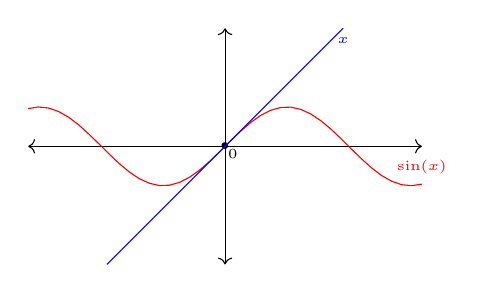
\begin{tikzpicture}[domain=-5:5, scale=0.5]
%\draw[very thin,color=gray] (-0.1,-1.1) grid (3.9,3.9);
\draw[<->]   (-5,0) -- (5,0);
\draw[<->] (0,-3) -- (0,3); % node[above] {$f(x)$};

   \node at (0.2,-0.2){\tiny$0$};
      \node at (0,0){\tiny$\bullet$};

%
\draw[color=red, domain=-5:5, samples=40] plot (\x, {sin(\x r)} ) node[above] {\tiny$\sin(x)$};

\draw[color=blue, domain=-3:3, samples=40] plot (\x,{\x  } ) node[below] {\tiny$x$};


\end{tikzpicture}$}
}
\caption{\small $\sin(x)$ and $x$ are very close around 0, but their distance diverges at $\pm \infty$.}
\label{fig:sinid1}
\end{subfigure} \ \ \ 
\begin{subfigure}{0.48\textwidth}
\parbox[h][3.5cm][c]{\textwidth}{
\adjustbox{center}{$
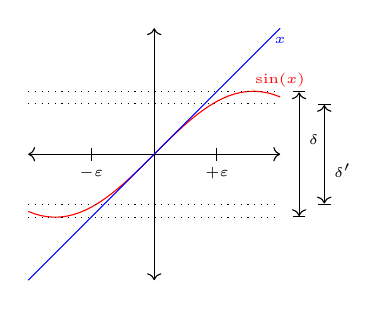
\begin{tikzpicture}[domain=-2:2, scale=0.8]
%\draw[very thin,color=gray] (-0.1,-1.1) grid (3.9,3.9);
\draw[<->]   (-2,0) -- (2,0);
\draw[<->] (0,-2) -- (0,2); % node[above] {$f(x)$};


\draw[|-|] (-1,0) -- (1,0);
\node(r) at (-1,-0.3) {\tiny$-\varepsilon$};
\node(r) at (1,-0.3) {\tiny$+\varepsilon$};
   % \node at (0,0)[circle,fill,inner sep=1pt]{};
%
\draw[color=red, domain=-2:2, samples=40] plot (\x, {sin(\x r) } ) node[above] {\tiny$\sin(x)$};

\draw[color=blue, domain=-2:2,samples=40] plot (\x,{\x  } ) node[below] {\tiny$x$};


\draw[dotted] (-2,1) -- (2,1);
\draw[dotted] (-2,-1) -- (2,-1);

\draw[dotted] (-2,0.8) -- (2,0.8);
\draw[dotted] (-2,-0.8) -- (2,-0.8);

\draw[|<->|] (2.3,1) -- node[above right]{\tiny$\delta$} (2.3,-1);
\draw[|<->|] (2.7,0.8) -- node[below right]{\tiny$\delta'$} (2.7,-0.8);


\end{tikzpicture}$}
}
\caption{\small The self-distances $\delta,\delta'$ of $\sin(x)$ and $x$ in a small interval $[-\varepsilon,\varepsilon]$ of $0$ are very close.}
\label{fig:sinid2}
\end{subfigure}
\caption{The sup-distance is inadequate for contextual transformations.}
\label{fig:sinid}
\end{figure}
 
  While several frameworks  have been developed for contextual reasoning \cite{10.1145/1932681.1863568,Gaboardi_2013,Azevedo_de_Amorim_2017,chaudhuri, dallago:differential-stlc},  these approaches seem to suggest that lifting an account of program
differences in terms of program metrics to a fully higher-order language still constitutes a major challenge. 
%Yet, in this paper we propose a framework which accommodates both aspects.
%
% The question that motivates this paper is whether a notion of program difference of this kind can itself be seen as a metric over the programs of a programming language with higher-order types.  
Suppose to start from a language  containing a type $\mathsf{Real}$ for real numbers on which errors are measured with the standard metric. It is not clear, then, how to lift this metric to higher-order types, \emph{e.g.}~to $\mathsf{Real}\to \mathsf{Real}$, so that distances are measured in a contextual way.



A standard solution is to take the sup-distance, that is, to let, for $f,g:\mathsf{Real}\to \mathsf{Real}$, $d(f,g)=\sup\{d(f(r),g(r))\mid r\in \mathsf{Real}\}$. This solution works well in models in which programs are interpreted as \emph{non-expansive} or \emph{Lipschitz-continuous} maps \cite{Hofmann2014, Azevedo_de_Amorim_2017}. However, as is well-known, such models are not \emph{cartesian-closed}\footnote{In fact, cartesian closed categories of metric spaces and non-expansive functions \emph{do} exist \cite{Escardo1999, Stubbe2009}, but, to our knowledge, none of these categories contains the real numbers with the standard metric.}, so they do not account for 
 the simply-typed lambda-calculus in its full generality, but only for linear or sub-exponential variations of it (such as $\mathsf{Fuzz}$ \cite{10.1145/1932681.1863568,Gaboardi_2013,Azevedo_de_Amorim_2017}).
 Also, it has been shown \cite{10.1109/LICS.2015.64} that in a probabilistic setting the non-linearity of higher-order programs has the effect of \emph{trivialising} metrics, that is, of forcing distances to be either 0 or 1, hence collapsing program distances onto usual notions of program equivalence.
Most importantly, even if one restricts to a sub-exponential language, the sup-distance seems inadequate to account for contextual transformations as the replacement of $\lambda x.\sin(x)$ by $\lambda x.x$ around 0,  as the sup-distance between such programs is infinite (see Fig. \ref{fig:sinid}). 
 
 
On the other side of the coin, other approaches like \cite{chaudhuri, dallago:differential-stlc} are fully contextual and higher-order, but provide, at best, only weak approximations of a standard notion of metric.  
 Nonetheless, these approaches introduce the idea, that we retain here, that program differences must be taken as being themselves some kind of programs, relating errors in input with errors in  output,  and separate programs accordingly in two different classes: \emph{exact} programs, computing mappings from well-defined inputs to well-defined outputs, and \emph{approximate} programs, computing mappings from errors in the input to errors in the output.
%

%
%way to lift a metric $d$ on a set $A$ to a set of functions from $B$ to $A$ is by letting the distance between  be defined as the sup of the distances $d(f(x),f(x))$, with $x$ ranging on $B$.
%This approach is at work in several frameworks
%
%
%A standard way to measure differences between programs is by means of program metrics, that is, by endowing types $A$ with a distance $d:A\times A\to \mathbb R^{+}$. However, program metrics usually fail our compositional demand. Typically, in such models the distance between two programs $f,g: \mathsf{Real}\to \mathsf{Real}$ is computed as the $\sup$ of the distances between the values $f(r)$ and $g(r)$, for $r$ a ground element of $\mathsf{Real}$. 
%This approach is then not fine enough to capture differences which might depend on the context. For instance, whenever $g$ is obtained from $f$ by a truncated Taylor expansion around a point $r$, or by the replacement of a  $\mathsf{while}$ loop in $f$ by its perforation, the $\sup$-distance between $f$ and $g$ will most likely be infinite.
%
%
%A second issue with program metrics is that devising models of higher-order programming languages in which types are metric spaces still remains a non-trivial task. In fact, it is well-known that usual categories of metric spaces (\textit{e.g.} those generated by \emph{Lipschitz-continuous} functions)
%%\footnote{An exception is the metric model of PCF in \cite{Escardo1999}, based on a cartesian closed category of \emph{ultrametric spaces}, which in particular excludes $\R$.} \cite{Hofmann2014}) 
%are not \emph{cartesian-closed}, that is, do not provide models of the simply-typed lambda-calculus, but only of linear or sub-exponential variations of it (such as the system $\mathsf{Fuzz}$ \cite{10.1145/1932681.1863568,Gaboardi_2013,Azevedo_de_Amorim_2017}).
%
%
%; 


%second, such models are not at first sight compatible with the compositional approach advocated above: in a metric model the distance between two functional program is a real number (e.g. the max of the distances between the inputs), and this hardly provides a good compositional notion of difference [EXAMPLE HERE, e.g. sin/id, highlight the role of context, you can't justify contextual transformations].

%EXAMPLE: Newton's approximation works well around some point (so it is contextual) -- see Di Cosmo Tweet on Apollo 11






\subparagraph*{Diameter Spaces}



In this paper we introduce a class of higher-order denotational models, that we call \emph{diameter space models}, to reason about program similarity and approximate program transformations.
In such models a higher-order type $A$ is interpreted as a 4-tuple $(|A|, \intervals{A}, \distances{A}, \diam_{A})$ called a \emph{diameter space}, where $|A|$ is a set of \emph{exact} values, $\intervals{A}\subset \mathcal P(|A|)$ is a complete lattice of \emph{approximate} values, $\distances{A}$ is a \emph{quantale}, and $\diam_{A}: \intervals{A}\to \distances{A}$ is a function, called \emph{diameter}, which provides a quantitative measure of approximate values.





The maps $\diam_{A}$ take their name from the fact that they  
 generalize some properties of the diameter function of the standard metrics on real numbers, in particular, 
the fact that the diameter is \emph{modular} over intersecting intervals (see Fig. \ref{fig:modular}).
Moreover, just like the standard metric on $\mathbb R$ can be recovered from the diameter by $d(x,y)=\mathsf{diam}([x,y])$, the function $\diam_{A}$ induces a \emph{generalized partial metric} $d_{A}:|A|\times |A|\to \distances{A}$ by letting $d_{A}(x,y)=\diam_{A}(x\vee y)$. 


Generalized partial metric spaces (henceforth GPMS) are a well-investigated class of metric spaces that has been widely applied in program semantics \cite{bkmp:partial-metrics, Bukatin1997, doi:10.1111/j.1749-6632.1994.tb44144.x, Schellekens2004, Samet:2013aa, Stubbe2018, HE201999}. 
Such spaces generalize standard metric spaces in that distances
need not be real numbers, but can be functions or any other type of object that leaves in a suitable \emph{quantale} \cite{Hofmann2014}, and \emph{self-distances} $d(x,x)$ need not be $0$ (which in turn leads to strengthen the usual triangular inequality as $d(x,y) + d(z,z)\leq d(x,z)+d(z,y)$).
%\footnote{The adjective ``partial'' comes from the fact that in partial metric semantics like \cite{} the  programs with a non-zero self-distance are those which are not total, in the sense of Scott domains. This will not be the case in our framework. 
%}   
%Observe that not only any standard metric space is a GPMS, but from from any partial metric $d$ one can retrieve a (generalized) metric $d'$ by letting $d'(x,y)=2d(x,y)-d(x,x)-d(y,y)$.


\begin{figure}
\adjustbox{center}{
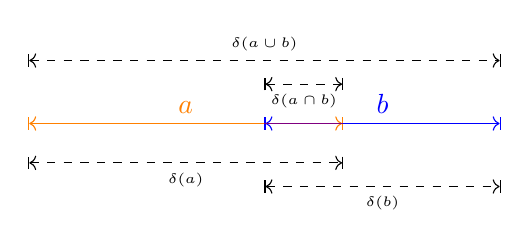
\begin{tikzpicture}


\draw[|<->|, orange] (-2,0) to node[above] {$a$} (2,0);
\draw[|<->|, blue] (1,0) to node[above]  {$b$} (4,0);
\draw[violet] (1,0) to (2,0);

\draw[|<->|, dashed] (-2,0.8) to node[above] {\tiny$\delta(a\cup b)$} (4,0.8);
\draw[|<->|, dashed] (1,0.5) to node[below] {\tiny$\delta(a\cap b)$} (2,0.5);
\draw[|<->|, dashed] (-2,-0.5) to node[below] {\tiny$\delta(a)$} (2,-0.5);
\draw[|<->|, dashed] (1,-0.8) to node[below] {\tiny$\delta(b)$} (4,-0.8);



\end{tikzpicture}}
\caption{\small The diameter function is \emph{modular} over intersecting real intervals: 
$\mathsf{diam}(a\cup  b)+\mathsf{diam}(a\cap b)=\mathsf{diam}(a)+\mathsf{diam}(b)$ for all $a,b\in [\R]$ such that $a\cap b\neq \emptyset$.
This property is at the heart of our generalization of diameters.}
\label{fig:modular}
\end{figure}


%
%
%In this paper we show that the standard metric on real numbers can be lifted to higher-order types in a novel way, yielding a metric semantics of the simply typed lambda-calculus in which types are interpreted as quantale-valued partial metric spaces. Noticeably, the distances between objects of higher-types are elements of functionals, thus non-numerical, quantales,. This on the one hand allows us to faithfully model arbitrary functions, thus deviating from classic metric semantics, and on the other enables contextual reasoning. 
%
%%The partial metrics induced by diameter spaces 
%% generalize some properties of the standard metric on real numbers: the fact that the distance between two points $x,y$ coincides with the diameter of the smallest \emph{interval} containing them, 
%%as well as the fact that the diameter is a \emph{quasi-modular} function (i.e. it satisfies $\mathsf{diam}(a\cup b)+\mathsf{diam}(a\cap b)= \mathsf{diam}(a)+\mathsf{diam}(b)$, for all intersecting intervals $a,b$, see Fig. \ref{fig:modular}).
%%
%While diameter spaces generalize the standard metric of real numbers, unlike the latter, they scale well from reals to real-valued functions. In particular, 
%we show how to construct a diameter space over the set of programs of type $\mathsf{Real}\to \mathsf{Real}$. This space induces then a partial metric on such programs in which  
%
%, in which approximate values are sets of programs $t$ induced by some $\mathsf{Real}$-indexed family of intervals $I$, i.e. such that for all real $r$, $t(r)\in I(r)$. In this way, any two (exact) programs $t,u: \mathsf{Real}\to \mathsf{Real}$ generate a smallest approximate program $t\vee u$ (namely, the set of those $v$ such that, for all $r$, $v(r)$ is in the interval generated by $t(r)\vee u(r)$), and the induced distance between $t$ and $u$ is the map (living in a suitable quantale) that associates a 
%
%%
%%%In any metric space the distance can be recovered from the diameter function\footnote{We recall that in any metric space $(X,d)$ one can define a map $\mathsf{diam}: \mathcal P(X)\to \mathbb R^{+\infty}$ by $\mathsf{diam}(a)=\sup\{d(x,y)\mid x,y\in a\}$.} by $d(x,y)=\mathsf{diam}(\{x,y\})$. Similarly, 
%%%NO! QUI PARLA DI COME GENERALIZZI A R->R PROPRIETA DI R.
%%The choice to consider the distance between two functional programs like $\lambda x.\sin(x)$ and $\lambda x.x$ as being itself some kind of function leads naturally towards GPMS. Firstly, because it  implies that distances cannot be real numbers. Instead,
%In our model, we define  

\subparagraph*{New Ways of Measuring Distances between Programs of Functional Type}
% measure distances on $\mathsf{Real}\to\mathsf{Real}$}

In our model, 
the distance between  two programs $f,g:\mathsf{Real}\to \mathsf{Real}$ lives in the functional quantale of monotone maps from \emph{approximate values} of $\mathsf{Real}$ (\emph{i.e.} closed intervals) to positive reals. This function associates a closed interval $a$ with the diameter of the smallest interval containing \emph{both} $f(a)$ and $g(a)$. 
Observe that, with this definition,  the distance of $f$ \emph{from itself} needs not be (constantly) 0. Rather, it  provides a measure of the sensitivity of $f$, since it associates each interval $a$ with the size of the interval $f(a)$ spanned by $f$ on $a$. %For instance, the self-distance of $\lambda x.\sin(x)$ associates any interval $a$ with a value $\leq 2$ (the diameter of $\sin(a)$).


% Observe that this implies that, unless $t$ is constant, its distance from itself cannot be constantly 0.
%By contrast, the distance  between $t$ and $u$ yields a way to measure the sensitivity of the smallest approximation of \emph{both} $t$ and $u$. 

%This new metric 


The use of partial metrics with functional distances yields a rich and expressive framework to reason about  
contextual transformations. For instance, we can express the closeness of $\lambda x.\sin(x)$ and $\lambda x.x$ around 0 by the fact that their distance, applied to a small interval $[-\epsilon,\epsilon]$ of 0, is very close to the {self-distance} of
$\lambda x.\sin(x)$ on the same interval (as illustrated in Fig. \ref{fig:sinid2}). Moreover, we also show how the triangular inequality of partial metrics can be used to infer new bounds from previously established ones in a compositional way.

%. In other words, the interval spanned by both the sine and the identity function on $ [-\epsilon,\epsilon]$ almost coincides with the one spanned by 
%$\lambda x.\sin(x)$ alone 
%
% values which are close to those obtained by  $\lambda x.\sin(x)$ alone.

%
%
% two functions around 0 as the fact that 
%
%, when applied to a small interval of 0, will provide values which are close to those provided by the 
%
%meaning that the 
%
%
%
%describes the fact that these two programs are very similar around 0, since  the fact that the interval spanned by \emph{both} the sine and the identity function, when applied to a small interval of 0, almost coincides with the interval spanned by the sine function alone (see Fig. \ref{fig:sinid}).
%
%
%Observe that with this definition the distance of $\lambda x.\sin(x)$ from itself cannot be constantly 0. In fact, in our model, 
% self-distances of functional programs will play a role similar to derivatives, in particular, 
% 
% $ d_{\mathsf{Real}\to\mathsf{Real}}(f,f)$ is constantly 0 only if $f$ is constant. %, 
%
%
%
%This notion of distance is 
%with contextuality
%
%This definition implies then that the \emph{self-distance} of $\lambda x.\sin(x)$ (resp. $\lambda x.x$)  is not constantly 0; instead, it associates each interval $a$ with a value $\leq 2$ (resp. with $\diam(a)$, see Fig: \ref{fig:sinid}). Indeed, as this example suggests, the self-distances of functional programs behave as sort of derivatives, in particular, $ d_{\mathsf{Real}\to\mathsf{Real}}(f,f)$ is constantly 0 only if $f$ is constant. %, and moreover self-distances 
% %compose through a (lax) chain-rule.
%
%This notion of functional distance 
%While the fact that replacing  $\lambda x.\sin(x)$ by $\lambda x.x$, when applied close to 0 yields a negligible change cannot be expressed in a metric semantics based on the sup-distance, in our framework this will be expressed by the fact that their distance, computed in an interval around $0$ with a small enough diameter, is very close to the \emph{self-distance} of $\lambda x.\sin(x)$ (see Fig. \ref{fig:sinid}). 
%
%





%The main two technical contributions of this paper are the following. First, we show that the construction just sketched actually permits to scale the standard  metric for $\mathsf{Real}$ to higher-order types, yielding a partial metric model of a simply typed $\lambda$-calculus with a type of real numbers.
%
\subparagraph*{Diameter Space over a Cartesian Closed Category}
While our construction was though to account for rather concrete examples of transformations (e.g. the sine/identity transformation or loop perforation), diameter spaces can be constructed starting from any higher-order programming language with a reasonable denotational semantics. In fact, for \emph{any} cartesian closed category $\mathbb C$, we can construct a cartesian \emph{lax-}closed category $\dsp(\mathbb C)$, whose morphisms can be seen as approximate versions  of the morphisms of $\mathbb C$. The ``lax'' preservation of the cartesian closed structure reflects the fact that, by composing approximations in a higher-order setting, also their error rates compose (typically, approximating non $\beta$-normal $\lambda$-terms will lead to higher error-rates than approximating their $\beta$-normal forms). 



The generality of our construction shows in particular that our partial metric semantics requires no restrictions (\textit{e.g.} Lipschitz-continuity) on morphisms, and adapts well to the model one starts with: for instance, in the category $\dsp(\set)$ we obtain a partial metric on the set of \emph{all}  set-theoretic functions from $\mathbb R$ to $\mathbb R$, while the models $\dsp(\eff)$ (where $\eff$ is the \emph{effective topos} \cite{hyland:effective-topos}) and $\dsp(\scott)$ show that our approach scales well to a more computability-minded setting.


%The step from $\mathbb C$ to $\mathsf{Diam}(\mathbb C)$ preserves the cartesian closed structure in a \emph{lax} way: this reflects the fact that,


%
%
%      
%\subparagraph*{Interval spaces over your favorite higher-order language }
%
%
%%While our framework retains several aspects from existing frameworks for program approximations (\cite{}), it is the first one to provide a clear connection with standard techniques for program metrics. Moreover, 
%Beyond establishing a connection with program metrics, our approach has the advantage of being \emph{language-independent}: To demonstrate this fact we show how to construct, from an arbitrary cartesian closed category $\mathbb C$, an interval space model $\mathcal I(\mathbb C)$ in which exact programs coincide with the arrows in $\mathbb C$. %

%
%which combines both qualitative and quantitative information on $\sigma$. The first two components of $A$ are a set $|A|$ of \emph{exact} programs and a complete lattice $\intervals{A}$ of \emph{approximate} programs.
%
%
%[GPMSs exact/approximate
%The quantitative part can be seen as either a measure on approx. programs or a distance on exact programs
%]
%
%[Generality: categoricity, no restriction on functions]
%
%
%- explain GPMSs
%
%- discuss DMs
%
%- derivative?
%
%
%In such models higher-order types are endowed with the structure of a 
%\emph{generalized partial metric space} (GPMS),
%
%
%
%We recall that a \emph{generalized} metric space is one in which distances need not be measured on the usual quantale of positive reals but over an arbitrary quantale. 
%
%
%The idea of considering program distances as programs themselves forced us to 
%generalize the usual notion of metric space in two directions.
%
% 
%%
%%
%% $|A|$  exact programs in $\sigma$, while $\mathcal I$ is a complete sublattice of $\mathcal P(A)$ whose elements are called \emph{intervals}, and codify approximate programs from $\sigma$. A map of interval spaces similarly comprises both an exact map between points and an approximate (monotone) map between intervals.
%The last two components provide quantitative information on exact and approximate programs:
%$\distances{A}$ is a (commutative and integral) quantale and $\diam_{A}: \intervals{A}\to \distances{A}$ is a function, called \emph{diameter}, which measures the largeness of approximations. 
%
%
%[HERE INTUITION ABOUT DIAMETER]
%
%For the reasons spelled above, whenever we consider intervals over functional programs, the measure of an interval should not be taken in the standard quantale of positive reals. This is why the quantale $\mathbb Q$ may vary across different interval spaces. For example, to measure an interval $a$ of programs from $\mathsf{Real}$ to $\mathsf{Real}$, we will let $\mathbb Q$ be the quantale of monotone maps from real intervals to $\mathbb R^{+\infty}$, and let $\delta(a)$ be the map associating a real interval $b$ with the maximum distance between $f(x),g(y)$, where $x,y\in b$ and $f,g\in a$.  
%
%A fundamental property of the quantitative measure $\delta$ is that it can be equivalently described through a program metric. In fact, by composing $\delta$ with the map associating two exact programs with their least common approximation, one obtains a \emph{partial metric} $d: A\times A \to \mathbb{Q}$ such that the measure $\delta(a)$ of an interval can be computed as the \emph{diameter} of $a$ (that is, as $\sup\{d(x,y)\mid x\in a\}$).
%%
%%by composing $\delta$ with the map $\vee$ associating two exact programs with their least common approximation, we obtain a binary map over exact programs $d= \vee\circ \delta: A\times A\to \mathbb{Q}$, which is in fact a \emph{partial metric}.
%
%
% Partial metrics are a well-investigated class of metrics which is widely applied in program semantics \cite{bkmp:partial-metrics, doi:10.1111/j.1749-6632.1994.tb44144.x, Samet:2013aa}. 
%Such metrics generalize usual metrics by not requiring self-distances to be $0$ (and modifying the triangular law accordingly).
%The appeal to partial metrics was indeed forced on us by compositionality: when $f$ is a functional program, its self-distance $d(f,f)$ must itself be a function relating changes in the input of $f$ with changes in its output, hence a function $f$ such that $d(f,f)$ is constantly $0$ would be one which is not sensitive to its input at all or, in other words, a constant function.   


%[MODIFY WHEN EXAMPLES ARE CLEARER] While being based on a general categorical construction, interval spaces adapt well to the specific features of each language. We show that the approximate programs defined for a specific language L incorporate the features of L, since specific interval structures can be defined starting from programs of L by a pullback operation.
%For instance, if L has a derivative or finite difference operator $\Delta$, then by pulling back over it we can define an interval structure over $\mathsf{Real}\to \mathsf{Real}$ so that the difference between two programs depends, in addition to their behavior, on the behavior of their derivatives.



\section{Generalized partial metric spaces}





Partial metric spaces were  introduced in the early nineties as a variant of metric spaces in which self-distances can be non-zero. Such spaces have attracted much attention in program semantics
\cite{bkmp:partial-metrics, Bukatin1997, doi:10.1111/j.1749-6632.1994.tb44144.x, Schellekens2004, Samet:2013aa, Stubbe2018, HE201999}, due to their compatibility with standard constructions from both domain theory (since their topology is $T_{0}$) and usual metric topology (\textit{e.g.} Cauchy sequences, completeness, Banach-fixed point theorem) \cite{bkmp:partial-metrics, doi:10.1111/j.1749-6632.1994.tb44144.x}.
\emph{Generalized partial metric spaces}, \textit{i.e.} partial metric spaces whose metric takes values over an arbitrary quantale \cite{Hofmann2014}, are well-investigated too \cite{AGT2000,AGT7849}. 

In this paper we will only be concerned with partial metrics taking values over a \emph{commutative integral} quantale \cite{Hofmann2014}, of which we recall the definition below.
% (which is the only kind of quantale we will consider here): %, as we will use these concepts throughout this paper.

\begin{definition} A \emph{commutative integral quantale} is a triple $(Q, \quantaleop, \quantalegeq)$ where:
\begin{itemize}
\item $(Q, \quantalegeq)$ is a complete lattice,
\item $(Q, \quantaleop)$ is a commutative monoid,
\item $\quantaleop$ commutes with arbitrary $\inf$s,
\item the least element of $Q$ is neutral for $\quantaleop$.
\end{itemize}
\end{definition}

For readability, we have we have reversed the ordering with respect to the conventional definition, so that for example, $([0,\infty], +, \leq)$ is a commutative integral quantale whose least element is $0$  (as opposed to ``$([0,\infty], +, \geq)$ is a commutative integral quantale whose \emph{largest} element is $0$'', which is what we would get with the usual definition). It is straightforward to check that for all commutative integral quantales $Q,R$, the product monoid $Q \times R$ equipped with the product ordering is also a commutative integral quantale. In addition, for all posets $X$, the set of monotone functions from $X$ to $Q$, equipped with the pointwise monoid operation and the pointwise ordering, is also a commutative integral quantale. Another example of commutative integral quantale is given by the lattice of ideals of any commutative ring, with the product of ideals as the monoid operation.


We recall now the definition of a generalized partial metric space:


\begin{definition} A \emph{generalized partial metric space} (in short, GPMS) is the data of a set $X$, a commutative integral quantale $Q$ and a function $d : X \times X \to Q$ such that: \begin{itemize}
\item for all $x,y \in X$, $d(x,x) \quantalegeq d(x,y)$,
\item for all $x,y \in X$, if $d(x,x) = d(x,y) = d(y,y)$, then $x = y$,
\item for all $x,y \in X$, $d(x,y) = d(y,x)$,
\item for all $x,y,z \in X$, $d(x,z) \quantaleop d(y,y) \quantalegeq d(x,y) \quantaleop d(y,z)$.
\end{itemize}
\end{definition}

For every metric space $(X,d)$, the structure $(X, ([0,\infty], +, \leq), d)$ is a GPMS. 
As is well-known \cite{bkmp:partial-metrics}, any real-valued GPMS $(X,[0,\infty],d)$ induces a metric $d^{*}$ by letting 
\begin{equation}\label{eq:pmettomet} % Only works with a division quantale, e.g. [0,\infty]
d^{*}(x,y)=2d(x,y)-d(x,x)-d(y,y)\tag{$\star$}
\end{equation}


For a more telling and somewhat archetypal example, take any set $X$ and consider the set $X^{\leq \omega}$ of all sequences of elements of $X$ indexed by an ordinal less than or equal to $\omega$. For all such sequences $s,t$, let $d(s,t) = 2^{-n} \in [0,\infty]$, where $n$ is the length of the largest common prefix to $s$ and $t$: one can check that $(X^{\leq \omega}, [0,\infty], d)$ is indeed a generalized partial metric space. In fact, if we interpret the prefixes of a sequence as pieces of partial information, then we have $d(s,s) = d(s,t)$ if and only if $t$ is a refinement of $s$ (\textit{i.e.} if it contains more information), and $d(s,s) = 0$ if and only if $s$ is total (\textit{i.e.} if it cannot be refined).

One can check that for all partial metric spaces $(X, Q, d_X)$ and $(Y, R, d_Y)$, $(X \times Y, Q \times R, d_{X \times Y})$ is a generalized partial metric space, where $d_{X \times Y}((x_1, y_1), (x_2, y_2)) = (d_X(x_1, x_2), d_Y(y_1, y_2))$. However, in general, it is not clear how one should define a partial metric on a function space. In  Section \ref{subsection:type-gpms} we introduce a construction to obtain partial metric spaces on function spaces by generalizing some properties of the standard diameter function on sets of real numbers.


\section{Approximate programs for the simply-typed $\lambda$-calculus with a type of reals}
\label{section:stlc}

% !TEX root = CSL 2021.tex

To illustrate our construction, we start from a relatively concrete example: we consider a simply-typed lambda calculus with a base type and primitives for real numbers, and we follow the plan outlined in the introduction, which yields for each simple type a notion of approximate value, approximate function, diameter and distance between programs. Most definitions are straightforward and intuitive: the interesting, not immediately obvious point is that our construction does yield a \emph{partial metric} on each type.

\emph{Simple types} are defined as follows: $\mathsf{Real}$ is a simple type; if $A$ and $B$ are simple types, then $A \to B$ and $A \times B$ are simple types.
For all $n>0$, we fix a set $\mathcal{F}_n$ of functions from $\mathbb{R}^n$ to $\mathbb{R}$. We consider the usual Curry-style simply-typed $\lambda$-calculus over the types defined above (the left and right projection are denoted by $\pi_L:A\times B \to A$ and  $\pi_R:A\times B \to B$ respectively, and the constructor for pairs by $\left\langle-,-\right\rangle$), enriched with the following constants: for all $r \in \mathbb{R}$, a constant $r:\mathsf{Real}$; for all $n>0$ and all $f\in\mathcal{F}_n$, a constant $f:\mathsf{Real}\to\ldots\to\mathsf{Real}\to\mathsf{Real}$. We call this calculus $\STLC$, and its terms are simply called \emph{terms}. We write $t[x_1 := u_1, \ldots, x_n := u_n]$ to denote the \emph{simultaneous} substitution of $u_1, \ldots, u_n$ for $x_1, \ldots, x_n$ in $t$. For all types $A$, we denote by $\Lambda_A$ the set of closed terms of type $A$. The relation of $\beta$-reduction is enriched with the following rule, extended to all contexts: for all $n>0$, $f\in\mathcal{F}_n$, and $r_1,\ldots,r_n\in\mathbb{R}$, $f r_1 \ldots r_n \to_\beta s$, where $s = f(r_1, \ldots, r_n)$. By standard arguments, this calculus has the properties of subject reduction, confluence and strong normalisation.

In addition to the usual notion of $\beta$-equivalence between terms of $\STLC$, we will exploit also a stronger equivalence: given two closed terms $t,u$ of type $A$,  we say that $t$ and $u$ are \emph{observationally equivalent} and write $t \oeq_A u$ if for all terms $C$ such that $x:A \vdash C : \mathsf{Real}$ is derivable, $C[x:=t]$ is $\beta$-equivalent to $C[x:=u]$ (which amounts to saying that they both $\beta$-reduce to the same real number).  It is clear that observational equivalence is a congruence and that two $\beta$-equivalent terms are always observationally equivalent. The notion of distance we define in the next paragraph will be a generalisation of this notion of equivalence.



\subsection{Approximate Values and Approximate Programs}

The first step of our construction for $\STLC$ is to associate to each simple type $A$ a set $\intervals{A}$ whose elements are certain sets of programs of type $A$ that we call \emph{approximate values of type $A$}. 
A closed term $t\in \Lambda_{A}$ represents a program with return type $A$ and no parameters, so an approximate value can be thought as a specification of a program with return type $A$ and no parameters \emph{up to} a certain degree of error or approximation.

For each simple type $A$, the set of approximate values $\intervals{A}\subseteq \mathcal P(\Lambda_A)$ is defined inductively as follows:
\begin{itemize}
\item $\intervals{\mathsf{Real}} = \{ \{ t \in \Lambda_\mathsf{Real} \mid \exists r \in I, t \to_\beta^* r \} \mid I \subseteq \mathbb{R} \text{ is a compact interval or $\emptyset$ or } \mathbb{R} \}$,
\item $\intervals{A \times B} = \{ a \times b \mid a  \in \intervals{A}, b \in \intervals{B} \}$, where $a \times b = \{ t \in \Lambda_{A \times B} \mid \pi_L t \in a \text{ and } \pi_R t \in b \}$,
\item $\intervals{A \to B} = \{ \{ t \in \Lambda_{A \to B} \mid \forall u \in \Lambda_{A},~ tu \in I(u) \} \mid I : \Lambda_A \to \intervals{B} \}$.
\end{itemize}

The approximate values of type $\mathsf{Real}$ are sets of closed programs of type $\mathsf{Real}$ which essentially coincide with the compact intervals of $\mathbb R$, plus the empty set and $\mathbb{R}$ itself. An approximate value in $\intervals{A\times B}$ is a ``rectangle'' $a \times b$, with $a\in \intervals{A}$ and $b \in \intervals{B}$, while an approximate value in $\intervals{A\to B}$ is uniquely determined by a function 
$I$ from closed terms $u\in \Lambda_{ A}$ to approximate values $I(u)\in \intervals{B}$.

For example, any two terms $t,u\in \Lambda_{\mathsf{Real}}$ with normal forms $q, r\in \mathbb{R}$ induce an approximate value $[t,u]_{\mathsf{Real}}= \{v\in \Lambda_{\mathsf{Real}}\mid  v\to_{\beta}^{*} s \land (q\leq s\leq r \vee q\geq s\geq r)\}$ of type $\mathsf{Real}$. Similarly, any two terms $t,u\in \Lambda_{\mathsf{Real}\to \mathsf{Real}}$ induce an approximate value
$[t,u]_{\mathsf{Real}\to \mathsf{Real}}= \{v\in \Lambda_{\mathsf{Real}\to\mathsf{Real}}\mid  
\forall r \in \Lambda_{\mathsf{Real}} \ vr\in [ tr, ur]_{\mathsf{Real}} 
\}$. For instance, if $t= \lambda x.\sin(x)+1$ and $u=\lambda x.\cos(x)-1$, then 
$[t,u]_{\mathsf{Real}\to \mathsf{Real}}$ contains all closed terms corresponding to maps oscillating between $\sin (x)+1$ and $\cos(x)+1$ (\textit{e.g.} the program $\lambda x. \sin(x+1)$, as illustrated in Fig. \ref{fig:interval1}).

\begin{figure}
%\begin{subfigure}{0.42\textwidth}
\parbox[h][3cm][c]{\textwidth}{
\adjustbox{center}{$
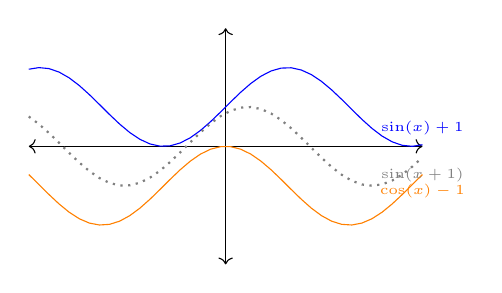
\begin{tikzpicture}[domain=-5:5, scale=0.5]
%\draw[very thin,color=gray] (-0.1,-1.1) grid (3.9,3.9);
\draw[<->]   (-5,0) -- (5,0);
\draw[<->] (0,-3) -- (0,3); % node[above] {$f(x)$};

   % \node at (0,0)[circle,fill,inner sep=1pt]{};
%
\draw[color=blue, samples=40] plot (\x,{sin(\x r)+1}) node[above] {\tiny$\sin(x)+1$};
\draw[color=orange, samples=40] plot (\x,{cos(\x r)-1}) node[below] {\tiny$\cos(x)-1$};

\draw[color=gray, dotted, thick, samples=40] plot (\x,{sin(deg(\x+1) ))}) node[below] {\tiny$\sin(x+1)$};


\end{tikzpicture}$}
}
\caption{$\lambda x.\sin(x+1)$ is in $[\lambda x.\sin(x)+1, \lambda x.\cos(x)+1]_{\mathsf{Real}\to\mathsf{Real}}$.}
\label{fig:interval1}
%\end{subfigure} \ \ \ 
\end{figure}


For all $A$, as a subset of $\mathcal{P}(\Lambda_A)$, $\intervals{A}$ is closed under arbitrary intersections and is therefore a complete lattice whose meet is given by intersection. In particular, for all $t\in\Lambda_A$, there is a least element of $\intervals{A}$ that contains $t$, which will be denoted by $\tointerval{t}$. 
One can check that $\tointerval{t} = \tointerval{u}$ if and only if $t\oeq_{A} u$.

Monotone functions from approximate values to approximate values represent \emph{approximate programs}. They behave like a model of the simply-typed $\lambda$-calculus in a weak sense, namely: \begin{itemize}
\item for all monotone functions $(\alpha_1, \ldots, \alpha_n) \mapsto c[\alpha_1, \ldots, \alpha_n] : \intervals{A_1} \times \ldots \times \intervals {A_n} \to \intervals {B \to C}$ and $(\alpha_1, \ldots, \alpha_n) \mapsto b[\alpha_1, \ldots, \alpha_n] : \intervals{A_1} \times \ldots \times \intervals {A_n} \to \intervals {B}$, we can define a monotone function $(\alpha_1, \ldots, \alpha_n) \mapsto (c[\alpha_1, \ldots, \alpha_n]~ b[\alpha_1, \ldots, \alpha_n]) = \sup\{\tointerval{vu} \mid v \in c[\alpha_1, \ldots, \alpha_n], u \in b[\alpha_1, \ldots, \alpha_n]\} : \intervals{A_1} \times \ldots \times \intervals {A_n} \to \intervals {C}$,
\item for all monotone functions $(\alpha_1, \ldots, \alpha_n) \mapsto c[\alpha_1, \ldots, \alpha_n] : \intervals{A_1} \times \ldots \times \intervals {A_n} \to \intervals {C}$ and all $i \leq n$, we can define a monotone function $(\alpha_j)_{j \neq i} \mapsto (\lambda \alpha_i.~ c[\alpha_1, \ldots, \alpha_n]) = \{ v \in \Lambda_{A_i \to C} \mid \forall t_i \in \Lambda_{A_i},~ v t_i \in c[\alpha_1, \ldots, \tointerval{t_i}, \ldots, \alpha_n] \} : \prod_{j \neq i} \intervals{A_j} \to \intervals{A_i \to C}$,
\end{itemize}
and these two constructions are weakly compatible with $\beta$-reduction and $\eta$-expansion:

\begin{proposition} \label{prop:intervals-weak-model-lambda} For all monotone functions $(\alpha_1, \ldots, \alpha_n, \beta) \mapsto c[\alpha_1, \ldots, \alpha_n, \beta] : \intervals{A_1} \times \ldots \times \intervals {A_n} \times  \intervals {B} \to \intervals {C}$ and $(\alpha_1, \ldots, \alpha_n) \mapsto b[\alpha_1, \ldots, \alpha_n] : \intervals{A_1} \times \ldots \times \intervals {A_n} \to \intervals {B}$, $$\begin{array}{ll} & (\alpha_1, \ldots, \alpha_n) \mapsto (\lambda \beta.~  c[\alpha_1, \ldots, \alpha_n, \beta])~ b[\alpha_1, \ldots, \alpha_n] \\ \leq & (\alpha_1, \ldots, \alpha_n) \mapsto c[\alpha_1, \ldots, \alpha_n, b[\alpha_1, \ldots, \alpha_n]]\text{,}\end{array}$$
and for all monotone functions $(\alpha_1, \ldots, \alpha_n) \mapsto d[\alpha_1, \ldots, \alpha_n] : \intervals{A_1} \times \ldots \times \intervals {A_n} \to  \intervals {B \to C}$,
$$\begin{array}{ll} & (\alpha_1, \ldots, \alpha_n) \mapsto \lambda \beta.~  d[\alpha_1, \ldots, \alpha_n]~ \beta \\ \geq & (\alpha_1, \ldots, \alpha_n) \mapsto d[\alpha_1, \ldots, \alpha_n]\text{,}\end{array}$$
where functions are ordered by pointwise inclusion.  In other words, on approximate programs, $\beta$-reduction and $\eta$-expansion \emph{discard} information, and conversely $\beta$-expansion and $\eta$-reduction \emph{recover} some information.
\end{proposition}

\begin{proof} Without loss of generality, we can assume $n=0$.
Let $v \in \lambda \beta.~ c[\beta]$ and $u \in b$. By definition, $tu \in c[\tointerval{u}]$, so $\tointerval{tu} \subseteq c[\tointerval{u}] \subseteq c[b]$. Therefore, $(\lambda \beta.~ c[\beta])~ b \subseteq b$.
Let $v \in d$. For all $u \in \Lambda_B$, by definition, $vu \in d\tointerval{u}$. Therefore, $v \in \lambda \beta.~ d~ \beta$.
\end{proof}

Beyond theoretical aspects (which will be made clearer in Section 5), 
Proposition \ref{prop:intervals-weak-model-lambda} is also important in practice because it implies that if we compute an approximation of a program from approximations of its parts and then simplify the resulting approximate program using $\beta$-reduction and $\eta$-expansion, what we obtain is still a valid approximation of the original program.


We can define a weak embedding from terms into approximate programs, by mapping each term to its tightest approximation: for all terms $t$ such that $\alpha_{1}:A_{1},\dots,\alpha_{n}:A_{n}\vdash t:B$, we define a monotone function $\partial(t):\intervals{A_{1}}\times \dots \times \intervals{A_{n}} \to \intervals{B}$ by $\partial(t)(a_1, \ldots, a_n) = \sup \{ \tointerval{t u_1 \ldots u_n} \mid u_1 \in \intervals{A_1}, \ldots, u_n \in \intervals{A_n} \}$. 

\begin{remark} \label{remark:push-exp-stlc}
The map $\partial$ is constant on classes of observational equivalence, and one can check that it is is weakly compatible with the constructions of the $\lambda$-calculus, in particular:
\begin{itemize}
\item $\partial (\alpha_{i})(a_{1},\dots, a_{n})=a_{i}$,
\item $\partial (tu)(a_{1},\dots, a_{n}) \subseteq \partial (t)(a_{1},\dots, a_{n}) ~ \partial (u)(a_{1},\dots, a_{n})$,
\item $\partial (\lambda \beta. t)(a_{1},\dots, a_{n}) \subseteq \lambda \beta.~ \partial (t)(\beta, a_{1},\dots, a_{n})$.
\end{itemize}
\end{remark}

This map $\partial(t)$ can be taken as a measure of the \emph{sensitivity} of $t$, as it maps an interval $a$, that is a quantifiably uncertain input, to a quantifiably uncertain output $\partial(t)(a)$. 
For instance, if we take the term $t[x]= \sin(x)+1$ above, then $\partial(t): \intervals{\mathsf{Real}}\to \intervals{\mathsf{Real}}$ sends the interval $[-\pi,\pi]_{\mathsf{Real}}$ into $[0,2]_{\mathsf{Real}}$.

\begin{figure}
%\begin{subfigure}{0.52\textwidth}
\parbox[h][3cm][c]{\textwidth}{
\adjustbox{center}{$
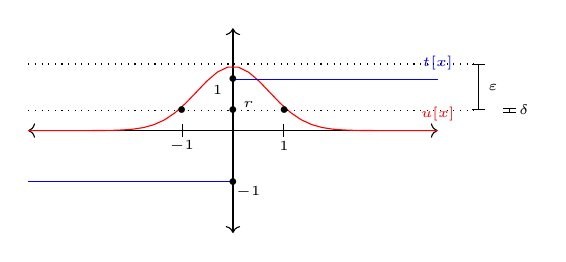
\begin{tikzpicture}[domain=-4:4, scale=0.65]

%\draw[very thin,color=gray] (-0.1,-1.1) grid (3.9,3.9);
\draw[<->]   (-4,0) -- (4,0);
\draw[<->] (0,-2) -- (0,2); % node[above] {$f(x)$};

\draw[dashed, |-|] (-1,0) -- (1,0);
\node(a) at (-1,-0.3) {\tiny$-1$};
\node(a) at (1,-0.3) {\tiny$1$};

\node(a) at (0.3,-1.2) {\tiny$-1$};
\node(a) at (-0.3,0.8) {\tiny$1$};
   % \node at (0,0)[circle,fill,inner sep=1pt]{};

\draw[|-|] (4.8,0.4) -- node[right] {\tiny$\varepsilon$} (4.8,1.3);

\draw[|-|] (5.4,0.35) -- node[right] {\tiny$\delta$} (5.4,0.45);


\draw[color=red, domain=-4:4, samples=40] plot (\x, {(1/2*sqrt(2*pi))*exp(-((\x)^2)) } ) node[above] {\tiny$u[x]$};
%\draw[color=violet, domain=-1.2:1.2] plot (\x, { (\x)^3 } );

\draw[color=blue, domain=-4:0] plot (\x,-1);
\draw[color=blue, domain=0:4] plot (\x,1) node[above] {\tiny$t[x]$};

\draw[dotted] (-4,0.4) -- (4.8,0.4);
\draw[dotted] (-4,1.3) -- (4.8,1.3);

\node(z) at (-1,0.4) {\tiny$\bullet$};
\node(zz) at (1,0.4) {\tiny$\bullet$};

\node(z) at (0,-1) {\tiny$\bullet$};
\node(zz) at (0,1) {\tiny$\bullet$};

\node(r) at (0,0.4) {\tiny$\bullet$};
\node(rr) at (0.3,0.5) {\tiny$r$};



\end{tikzpicture}$}
}
\caption{$\varepsilon=(\partial(u)\circ \partial(t))([-1,1])$ is bigger than $\delta=\partial(u\circ t)([-1,1])=[r,r]$.}
\label{fig:interval2}
%\end{subfigure}
\end{figure}

\begin{remark} \label{remark:oplax-functor-stlc}
When composing two maps $\partial(t)$ and $\partial(u)$, we might obtain a worse approximation than by computing $\partial(t[u/x])$ directly.
For instance, let $t[x]$ and 
$u[x]$ be, respectively, the discontinuous and Gaussian functions illustrated in Fig. \ref{fig:interval2}.  
If $a$ is the interval $[-1,+1]$, then $\partial(t)(a)=[-1,1]$, and since $u[x:=-1]=u[x:=1]\simeq_{\beta} r$ for some $0<r<1$, we deduce that $\partial(u)(\partial(t)(a))=[-1,1] \supsetneq [r,r  ]= \partial (u[t/x])(a)$.

\end{remark}










\subsection{A Partial Metric on Each Type}
\label{subsection:type-gpms}

We will now show how to associate to each type $A$ of $\STLC$ a generalised partial metric space $(\Lambda_{A}/\oeq_{A}, \distances{A}, d_{A})$. The definition of this space will exploit in an essential way the sets of approximate values $\intervals{A}$.


For all simple types $A$, we define a commutative integral quantale $(\distances{A}, \quantaleleq_A, \quantaleop_A)$ of \emph{distances of type $A$}:
\begin{itemize}
\item $(\distances{\mathsf{Real}}, \quantaleleq_\mathsf{Real}, \quantaleop_\mathsf{Real}) = ([0,\infty], \geq, +)$,
\item $\distances{A \times B} = \distances{A} \times \distances{B}$,
\item $\distances{A \to B} = \{ \text{monotonically decreasing functions from } \intervals{A} \text{ to } \distances{B} \}$.
\end{itemize}

Observe that the quantale $\distances{A\to B}$ is a set of functions over the approximate values of $A$.
For all simple types $A$, we now define a \emph{distance function} $d_A : \Lambda_A \times \Lambda_A \to \distances{A}$:
\begin{itemize}
\item $d_\mathsf{Real}(t,u) = \left\vert r-s \right\vert$, where $r,s$ are the unique elements of $\mathbb{R}$ such that $t \to_\beta^* r$ and $u \to_\beta^* s$,
\item $d_{A \times B}(t,u) = (d_A(\pi_L t, \pi_L u), d_B(\pi_R t, \pi_R u))$,
\item $d_{A \to B}(t,u) = a \mapsto \inf \left\{ d_B(rv, sw) \mid r,s \in \{t,u\}, v,w \in a \right\}$.
\end{itemize}



This distance is clearly compatible with observational equivalence (\textit{i.e.} if $a \oeq_A a'$ and $b \oeq_A b'$, then $d_A(a,b) = d_A(a',b')$). Our objective is now to prove that $\left(\Lambda_A/\oeq_A, \distances{A}, d_A\right)$ is a generalised partial metric space.


To this end, we define for all simple types $A$ a monotonically decreasing \emph{diameter function} $\diam_A : \intervals{A} \to \distances{A}$ by $\diam_A(a) = \inf \{ d_A(t,u) \mid t,u \in a \}$. As pointed out in the introduction, 
the name ``diameter'' refers to the fact that, as the standard diameter on the reals, the function $\diam_{A}$ is (almost) modular on intersecting approximate values, as we show in Proposition \ref{prop:submodular} below. 
 %-- or rather, using the quantale ordering convention, supermodular. 
 
 
 First, one can check that for all $t,u \in \Lambda_A$, $\diam_A\left(\tointerval{t} \vee \tointerval{u}\right) = d_A(t,u)$, and that:
\begin{itemize}
\item $\diam_\mathsf{Real}(a) = \sup\{s-r \mid s,r \in \mathbb{R} \text{ such that } s,r \in a\}$,
\item $\diam_\mathsf{A \times B}(p) = \left(\diam_A\left(\sup\left\{\tointerval{\pi_L t} \mid t \in p\right\}\right), \diam_B\left(\sup\left\{\tointerval{\pi_R t} \mid t \in p\right\}\right)\right)$,
\item $\diam_\mathsf{A \to B}(b) = a \mapsto \diam_B\left(\sup\left\{\tointerval{vt} \mid t\in a, v \in b\right\}\right).$
\end{itemize}

With that, we can prove that the diameter function $\diam_{A}$ is super-modular over intersecting approximate values: 
%``quasi-supermodularity'':
\begin{proposition}\label{prop:submodular} For all simple types $A$ and all $a,b \in \intervals{A}$ such that $a \wedge b \neq \emptyset$, $\diam(a \wedge b) \quantaleop \diam(a \vee b) \quantalegeq \diam(a) \quantaleop \diam(b)$.
\end{proposition}
\begin{proof}
We proceed by induction on types.

Let $a,b \in \intervals{\mathsf{Real}}$ such that $a\wedge b \neq \emptyset$. Let $I = \{r \in \mathbb{R} \mid r \in a\}$ and $J = \{s \in \mathbb{R} \mid s \in b\}$: then $I$ (respectively, $J$, $I \cap J$, $I \cup J$) is either $\mathbb{R}$ or a non-empty compact interval of $\mathbb{R}$, and its length in the usual sense is equal to $\diam_\mathsf{Real}(a)$ (respectively, $\diam_\mathsf{Real}(b)$, $\diam_\mathsf{Real}(a \wedge b)$, $\diam_\mathsf{Real}(a \vee b)$). Note that the only reason we know that $I \cup J$ is an interval is because $a\wedge b \neq \emptyset$ implies $I \cap J \neq \emptyset$. The length of an interval of $\mathbb{R}$ is equal to its Lebesgue measure, therefore $\operatorname{length}(I \cap J) + \operatorname{length}(I \cup J) = \operatorname{length}(I) + \operatorname{length}(J)$, so $\diam_\mathsf{Real}(a \wedge b) \quantaleop \diam_\mathsf{Real}(a \vee b) = \diam_\mathsf{Real}(a) \quantaleop \diam_\mathsf{Real}(b)$.

Let $a,b \in \intervals{A_L \times A_R}$ such that $a\wedge b \neq \emptyset$. For all $c \in \intervals{A_L \times A_R}$, let $c_L = \sup\{\tointerval{\pi_L t} \mid t \in c\}$ and $c_R = \sup\{\tointerval{\pi_R t} \mid t \in c\}$.
One can check that $(a \wedge b)_L = a_L \wedge b_L$, $(a \wedge b)_R = a_R \wedge b_R$, $(a \vee b)_L = a_L \vee b_L$ and $(a \vee b)_R = a_R \vee b_R$, so $\diam(a \wedge b) \quantaleop \diam(a \vee b) = (\diam(a_L \wedge b_L) \quantaleop \diam(a_L \vee b_L),  \diam(a_R \wedge b_R) \quantaleop \diam(a_R \vee b_R)) \quantalegeq (\diam(a_L) \quantaleop \diam(b_L), \diam(a_R) \quantaleop \diam(b_R)) = \diam(a) \quantaleop \diam(b)$.

Let $f,g \in \intervals{A \to B}$ and $a \in \intervals{A}$. For all $h \in \intervals{A \to B}$, let $ha = \sup\{\tointerval{vt} \mid v \in h, t \in a\}$. One can check that $(f \wedge g)a \subseteq (f a) \wedge (g a)$ and $(f \vee g)a = (f a) \vee (g a)$. As a result, $(\diam(f \wedge g)\quantaleop \diam(f \vee g))(a) \quantalegeq \diam((fa) \wedge (ga)) \quantaleop \diam((fa) \vee (ga)) \quantalegeq \diam(fa) \quantaleop \diam(ga) = (\diam(f)\quantaleop\diam(g))(a)$.
\end{proof}



\begin{corollary} \label{corollary:stlc-metric} For all simple types $A$, $\left(\Lambda_A/\oeq_A, \distances{A}, d_A\right)$ is a generalised partial metric space, that is to say:
\begin{enumerate}
\item for all $t,u \in \Lambda_A$, $d_A(t,t) \quantalegeq d_A(t,u)$,
\item for all $t,u \in \Lambda_A$, if $d_A(t,t) = d_A(t,u) = d_A(u,u)$, then $t \oeq_A u$,
\item for all $t,u \in \Lambda_A$, $d_A(t,u) = d_A(u,t)$,
\item for all $t,u,v \in \Lambda_A$, $d_A(t,v) \quantaleop d_A(u,u) \quantalegeq d_A(t,u) \quantaleop d_A(u,v)$.
\end{enumerate}
\end{corollary}
\begin{proof}
As mentioned above, for all $t,u\in\Lambda_A$, $d_A(t,u) = \diam_A(\tointerval{t} \vee \tointerval{u})$, which immediately gives point 3. Since $\delta_A$ is monotonically decreasing and $\tointerval{t} \vee \tointerval{t} \leq \tointerval{t} \vee \tointerval{u}$, we also get point 1.

One can check (by induction on types) that the restriction of $\diam_A$ to the ideal generated by the $\tointerval{t}$ (for $t \in \Lambda_A$) is \emph{strictly} decreasing. Therefore, if  $d_A(t,t) = d_A(t,u) = d_A(u,u)$, \textit{i.e.} $\diam_A(\tointerval{t}) = \diam_A(\tointerval{t} \vee \tointerval{u}) = \diam_A(\tointerval{u})$,  then $\tointerval{t} = \tointerval{t} \vee \tointerval{u} = \tointerval{u}$, so $t \oeq_A u$.

The triangular inequality is an immediate consequence of the quasi-supermodularity of $\diam_A$: $d(t,v) \quantaleop d(u,u) = \diam(\tointerval{t} \vee \tointerval{v}) \quantaleop \diam(\tointerval{u}) \quantalegeq \diam((\tointerval{t} \vee \tointerval{u}) \vee (\tointerval{u} \vee \tointerval{v})) \quantaleop \diam((\tointerval{t} \vee \tointerval{u}) \wedge (\tointerval{u} \vee \tointerval{v})) \quantalegeq \diam(\tointerval{t} \vee  \tointerval{u}) \quantaleop \diam(\tointerval{u} \vee  \tointerval{v}) = d(t,u) \quantaleop d(u,v)$.
\end{proof}


\begin{remark}
Corollary \ref{corollary:stlc-metric} is a slight refinement of the well-known fact \cite{6845021} that any 
function $\delta: L\to \mathbb R^{+\infty}$ on a lattice $L$ that is monotone and \emph{submodular}  (\emph{i.e.}~ satisfying $\delta(a\cup b)+ \delta(a\cap b) \leq \delta(a)+\delta(b)$ - recall that the order on $\mathbb R^{+\infty}$, taken as a quantale, is opposite to the usual order) induces a pseudo-metric $d: L\times L \to \mathbb R^{+\infty}$ by letting $d(a,b)=2\delta(a\vee b)-\delta(a)-\delta(b)$. In fact, one can decompose this construction: first, one defines a partial pseudometric $p$ on $L$ by $p(a,b) = \diam(a \vee b)$, and then $d$ is just the distance given by equation \eqref{eq:pmettomet}: $d(a,b) = p^*(a,b) = 2p(a,b)-p(a,a)-p(b,b)$.

 

\end{remark}


















\section{Computing program distances with partial metrics}

% !TEX root = CSL 2021.tex


In the previous section we showed how to associate each simple type $A$ with a  partial metric $d_{A}$ over the closed terms of type $A$. 
We  now illustrate through a few basic examples how the higher-order and metric features of this semantics can be used to formalize contextual reasoning about program differences.
To make our examples more realistic, we will consider some natural extensions of $\STLC$.

It is not difficult to see that all constructions from Section 3 scale well to any extension of $\STLC$ obtained by adding new base types. For example, we can add to our language a type $\mathsf{Nat}$ for natural numbers, indicating for each $n\in \mathbb N$, the corresponding normal forms of $\mathsf{Nat}$ as $\mathtt n$. A natural choice is to let   
$\intervals{\mathsf{Nat}}=\{ \{ t \mid \exists n\in a \ t\leadsto \mathtt n\}\mid a \text{ finite subset of }\mathbb N \text{ or }a=\mathbb N\}$, $\distances{\mathsf{Nat}}=\mathbb R^{+\infty}$ and $d_{\mathsf{Nat}}(t,u)=| n-m|$, where $t\to^{*}_{\beta}\mathtt n$ and $u\to^{*}_{\beta}\mathtt m$. 

Moreover, the constructions scale well also to extensions of $\STLC$ obtained by adding new program constructors, as soon as these do not compromise the normal form property (since the fact that closed programs of type $\mathsf{Real}$ have a normal form plays an important role in defining the set $\intervals{\mathsf{Real}}$).  
For instance, if we suppose that all programs of type $\mathsf{Real}\to\mathsf{Real}$ in $\STLC$ are either 
differentiable or integrable (see Remark \ref{rem:continuous}), we can consider extension of $\STLC$ with  differential or integral operators, as in $\mathsf{Real\ PCF}$ \cite{Di-Gianantonio:2013aa, Edalat:2000aa}.






\begin{example}[Taylor approximation]

We make the assumption that all programs of type $\mathsf{Real}\to\mathsf{Real}$ in $\STLC$ are differentiable and that for all $n$, we can define a term $\mathtt T^{n}: ((\mathsf{Real}\to \mathsf{Real})\times \mathsf{Real})\to \mathsf{Real}\to \mathsf{Real}$ such that $\mathtt T^{n}\langle f, r\rangle$ computes the $n$-th truncated Taylor expansion of $f$ at $r$. 
Then, given a term $t: \mathsf{Real}\to \mathsf{Real}$, the distance 
$d_{\mathsf{Real}\to\mathsf{Real}}(t, \mathtt T^{n}\langle t,\mathtt 0 \rangle)$ is the map associating an interval $a$ with the diameter of $t(a)\vee (\mathtt T^{n}\langle t,\mathtt 0 \rangle)(a)$. 
The difference between this value and the self-distance of $t$ will approximate 0 when $a$ is a small interval of $0$, and will tend to diverge when $a$ contains points which are far enough from 0. 

%between $t$ and its Taylor expansion within a context  $\mathsf C[\ ]= [\ ] r$ which applies them to some value $r$, can be computed as a function of the interval $[0,r]$.   
For example, if $t$ is the function $t=\lambda x.\sin(x)$, and $a$ is an interval of $0$, then using standard analytic reasoning we can compute a bound
$d_{\mathsf{Real}\to \mathsf{Real}}(t, \mathtt T^{n}\langle t,\mathtt 0 \rangle)(a  )\leq \frac{\diam_{\mathsf{Real}}(a)^{n+1}}{(n+1)!} $, which tends to $0$ as the diameter of $a$ tends to $0$.

Observe that if, instead, we used the $\sup$-distance $d_{\sup}(t,u)= \sup\{d_{\mathsf{Real}}(tr, ur)\mid r\in \Lambda_{\mathsf{Real}}\}$, then we could not reason as above since  
$d_{\sup}(\lambda x.\sin(x), \mathtt T^{n} \langle \lambda x.\sin(x),0\rangle)=\infty$ (as illustrated in Fig. \ref{fig:sintaylor}).  

We can use the higher-order structure of our semantics to push abstraction a bit further. For instance, we can define an approximate program 
$c[y_{1},y_{2}]=\left( \partial (\mathtt T^{n})\langle y_{1}, \tointerval{0}\rangle\right) y_{2}: \intervals{\mathsf{Real}\to \mathsf{Real}}\to \intervals{\mathsf{Real}}\to \intervals{\mathsf{Real}}$ which describes the sensitivity of the $n$-th Taylor expansions in 0. Given two programs $t$ and $u$ and a small interval $a$ of $0$, the real number $c[\partial(t)\vee \partial(u),a]$ measures how much the error of replacing the Taylor expansions of $t$ with the Taylor expansion of $u$ in $0$ diverges from the error produced by simply replacing  $t$ and $u$, when these are applied close to $0$. 
  
\end{example}

\begin{figure}
\begin{subfigure}{0.58\textwidth}
\parbox[h][3cm][c]{\textwidth}{
\adjustbox{center, scale=0.9}{$
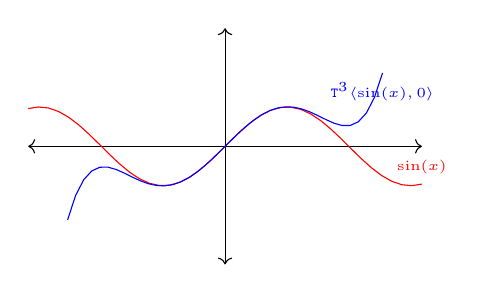
\begin{tikzpicture}[domain=-5:5, scale=0.5]
%\draw[very thin,color=gray] (-0.1,-1.1) grid (3.9,3.9);
\draw[<->]   (-5,0) -- (5,0);
\draw[<->] (0,-3) -- (0,3); % node[above] {$f(x)$};

   % \node at (0,0)[circle,fill,inner sep=1pt]{};
%
\draw[color=red, domain=-5:5, samples=40] plot (\x, {sin(\x r) } ) node[above] {\tiny$\sin(x)$};

\draw[color=blue, domain=-4:4, samples=40] plot (\x,{\x -((\x)^3)/6 + ((\x)^5/120  } ) node[below] {\tiny$\mathtt T^{3}\langle\sin(x),0\rangle$};


\end{tikzpicture}$}
}
\caption{\small The $\sup$-distance between $\sin(x)$ and its Taylor expansion $\mathtt T^{3}\langle\sin(x),0\rangle$ diverges.}
\label{fig:sintaylor}
\end{subfigure} \ \ \ 
\begin{subfigure}{0.4\textwidth}
\parbox[h][3cm][c]{\textwidth}{
\adjustbox{scale=0.45}{$\ \qquad\qquad
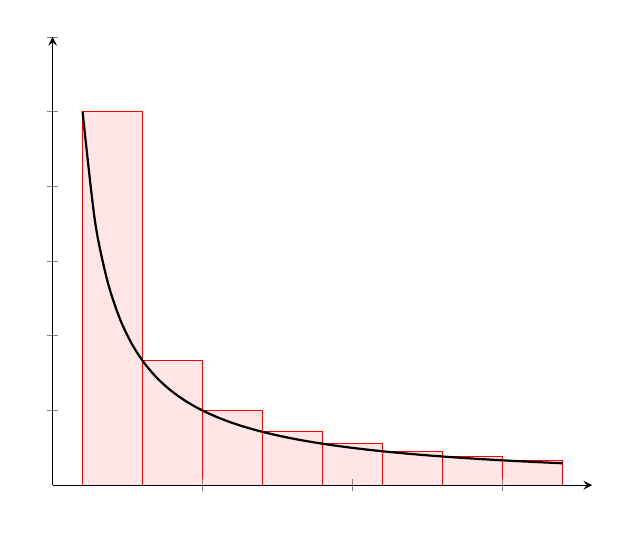
\begin{tikzpicture}
\begin{axis}[
    xticklabels={ , , },yticklabels={ , , },
    xmax=18,ymax=1.2,ymin=0,xmin=0,
    enlargelimits=true,
    axis lines=middle,
    clip=false,
    domain=0:17,
    axis on top
    ]

\addplot [draw=red, fill=red!10, ybar interval, samples=9, domain=1:17]
    {x^-1}\closedcycle;
%\addplot [draw=green, fill=green!10, ybar interval, samples=9, domain=17:1]
  %  {x^-1}\closedcycle;

\addplot[smooth, thick,domain=1:17,samples=40]{x^-1};

\end{axis}
\end{tikzpicture}
$}
%
%\begin{tikzpicture}[scale=0.7,
%    declare function={
%        f(\x)=2+sin(deg(\x-2))+sin(deg(3*\x))/2+sin(deg(5*\x))/8 + sin(deg(7*\x))/28;
%    }
%]
%\begin{axis}[
%    axis lines = middle,
%    %xtick ={1,1.5,2,2.5,3,3.5,4},
%    ytick ={0},
%    %xticklabels = {$a=x_0$,$x_1$,$x_2$,$x_3$, $\ldots$, $x_{n-1}$,$x_n=b$},
%    ymin = -0.2,
%    ymax = 3.7,
%    xmin = -0.2,
%    xmax = 5.2,
%    x=3cm,y=2cm,
%    axis line style = thick,
%    %xlabel={$x$},
%    %ylabel={$y$},
%    %extra x ticks={1.3,1.85,2.2,2.7,3.2,3.75},
%extra x tick labels={$\xi_1$, $\xi_2$, $\xi_3$, $\xi_4$, $\xi_{n-1}$, $\xi_n$},
%]
%
%\addplot [
%    domain=1:4,
%    samples=300,
%    line width=1pt,
%    fill=red, draw=none,
%    fill opacity=0.1
%] {f(x)} \closedcycle;
%
%\addplot [
%    domain=0:5,
%    samples=300,
%    line width = 1pt, red] {f(x)};
%
%\addplot [
%    ycomb, thick, red,
%    no markers,
%    samples at={1,1.5,...,4}
%] {f(x)};
%
%\addplot [
%    ycomb, thick, blue,
%    no markers,
%    samples at={1.3,1.85,2.2,2.6,3.2,3.65}
%] {f(x)};
%
%\addplot[ybar, bar width=30pt, domain=1:4,
%samples at={1.3,1.85,2.2,2.6,3.2,3.65}, fill=blue!50!cyan,fill opacity=0.3, draw=cyan]
%  {f(x)};
%
%
%\end{axis}
%\end{tikzpicture}$}
}
\caption{\small Definite integral $vs$ Riemann sums. \\ \   }
\label{fig:riemann}
\end{subfigure}
\caption{Computing bounds on distances: examples.}
\end{figure}


\begin{example}[Integral approximation]
We now assume that all functions in $\mathcal F_{n}$ are integrable and that we have (see \cite{Edalat:2000aa}) at our disposal a program $\lambda fx.\mathsf I_{[0,x]}(f): (\mathsf{Real}\to \mathsf{Real})\to \mathsf{Real}\to \mathsf{Real}$ such that $\mathsf I_{[0,r]}(t)$ computes (a precise enough approximation of) the definite integral $\int_{0}^{|r|}tx \ dx$.
In many contexts we might prefer to replace the expensive computation of $\mathsf I_{[0,r]}(t)$ by the (more economical but less precise) computation of a finite Riemann sum $\mathsf R^{n}_{[0,r]}(t)=  \sum_{i=1}^{n}(tx_{i})\cdot |r|/n$, where 
 $x_{i}=  i\cdot |r|/n$ (see Fig. \ref{fig:riemann}).  

%
%
%When the second derivative $D^{(2)}t$ of a program $t$ exists (and can be computed efficiently) and moreover is bounded by $M$ on $[0,r]$, the error of replacing the true integral  $\int_{0}^{r}tx dx$ (that we suppose $\mathtt I_{[0,r]}$ is close enough to) by its approximation through a finite Riemann sum, can be bounded
% as $d_{\mathsf{Real}}(\mathsf I_{[0,r]}t, \mathsf R^{n}_{[0,r]}t)\leq  M\cdot |r|^{3}/24n^{2}$.


Suppose now that, in order to approximate the integral of some computationally expensive program $t$ on $[0,r]$, we replace $t$ by some more efficient program $u$ which, over $[0,r]$, is very close to $t$. Let $\epsilon_{t}(r)$ indicate the distance between the true integral of $t$ over $[0,r]$ and $\mathsf{R}^{n}_{[0,r]}(t)$,
 and moreover let 
$\eta_{t,u}(r)$ be the diameter of $\partial(t)([0,r])\vee\partial(u)([0,r])$.

Using the metric structure of $\mathsf{Real}$ we can then bound the error we incur in by replacing the true integral \emph{of $t$} with the Riemann sum \emph{of $u$}. 
In fact, by standard calculation we can compute the bound
$d_{\mathsf{Real}} ( \mathsf{R}^{n}_{[0,r]}(t), \mathsf R^{n}_{[0,r]}(u))\leq 
d_{\mathsf{Real}\to\mathsf{Real}}(t, u)([0,r]) \cdot n \cdot |r|=\eta_{t,u}(r)\cdot n \cdot |r|$.
Then, using the triangular inequality of the standard metric on $\mathsf{Real}$ we deduce
\begin{align*}
 d_{\mathsf{Real}} ( \mathsf{I}_{[0,r]}(t), \mathsf R^{n}_{[0,r]}(u)) \leq
d_{\mathsf{Real}} ( \mathsf{I}_{[0,r]}(t), \mathsf R^{n}_{[0,r]}(t))  & +
d_{\mathsf{Real}} ( \mathsf{R}_{[0,r]}(t),\mathsf R^{n}_{[0,r]}(u)) \\
& \leq \epsilon_{t}(r)
+ 
\eta_{t,u}(r)\cdot 
 n\cdot |r|
 \end{align*}
 Using the partial metric on $\mathsf{Real}\to \mathsf{Real}$, we can also derive a bound expressing how much the error above is \emph{sensitive to changes of $r$}. 
First, using standard analytic techniques (under suitable assumptions for $t$ and its derivatives) one can find a program $v:\mathsf{Real}\to\mathsf{Real}$ such that $vr \to^{*}_{\beta}\epsilon_{t}(r)$. 
Then, using the triangular inequality of the partial metric on $\mathsf{Real}\to \mathsf{Real}$ we deduce, for all interval $a$, the following bound:
\begin{align*}
& d_{\mathsf{Real}\to\mathsf{Real}} (\lambda x. \mathsf{I}_{[0,x]}(t),\lambda x. \mathsf R^{n}_{[0,x]}(u))(a) \\
 &\leq \
d_{\mathsf{Real}\to\mathsf{Real}} ( \lambda x.\mathsf{I}_{[0,x]}(t), \lambda x.\mathsf R^{n}_{[0,x]}(t))(a) +
d_{\mathsf{Real}\to\mathsf{Real}} ( \lambda x.\mathsf{R}_{[0,x]}(t), \lambda x.\mathsf R^{n}_{[0,x]}(u))(a) \\
 & \qquad\qquad\qquad\qquad\qquad\qquad\qquad\qquad\qquad\qquad
- d_{\mathsf{Real}\to\mathsf{Real}} ( \lambda x.\mathsf{R}_{[0,x]}(t), \allowbreak \lambda x. \mathsf R^{n}_{0,x]}(t))(a) \\
 & \leq \ 
 %\Big(
d_{\mathsf{Real}\to \mathsf{Real}}(v,v)(a)
 %\diam_{\mathsf{Real}}(\partial(\lambda x.\epsilon_{t}(x))(y))
 +
 \big( d_{\mathsf{Real}\to\mathsf{Real}}(t,u)(a)- d_{\mathsf{Real}\to\mathsf{Real}}(t,t)(a)\big)\cdot n\cdot \diam_{\mathsf{Real}}(a)
 %\Big)
%  \bigg ( 
%\diam_{\mathsf{Real}}\Big ( \big (\partial(\mathsf I_{[0,\_]})\partial(t)y\big ) \vee \big (\partial(\mathsf I_{[0,\_]})\partial(u)y\big)\Big ) \\
% & \qquad\qquad\qquad\qquad\qquad\qquad
%+
%\big(\diam_{\mathsf{Real}} (\partial(t)(y)\vee \partial(u)(y))- \diam_{\mathsf{Real}} (\partial(t)(y))\big)\cdot n \cdot \diam_{\mathsf{Real}}(y)\bigg)
%% 
% \ ??(\varepsilon_{t})
%+ 
%(\partial(\eta_{t,u})(x)-\partial(\eta_{t,t})(x))\cdot 
% n\cdot \diam_{\mathsf{Real}}(x)
\end{align*}
\end{example}



%using the triangular inequality of partial metrics, we can deduce a bound for the distance 
%$ d_{\mathsf{Real}\to\mathsf{Real}} (\lambda x. \mathsf{I}_{[0,x]}t,\lambda x. \mathsf R^{n}_{[0,x]}u)\in \intervals{Real}\to \distances{Real}$ by 
%$d_{\mathsf{Real}\to\mathsf{Real}} (\lambda x. \mathsf{I}_{[0,x]}t,\lambda x. \mathsf R^{n}_{[0,x]}u)
%\leq
%d_{\mathsf{Real}\to\mathsf{Real}} ( \lambda x.\mathsf{I}_{[0,x]}t, \lambda x.\mathsf R^{n}_{[0,x]}t) +
%d_{\mathsf{Real}\to\mathsf{Real}} ( \lambda x.\mathsf{R}_{0,x]}t, \lambda x.\mathsf R^{n}_{0,x]}u) -
%d_{\mathsf{Real}\to\mathsf{Real}} ( \lambda x.\mathsf{R}_{0,x]}t,\lambda x. \mathsf R^{n}_{0,x]}t)
%\leq 
%\epsilon_{t,a}
%+ 
%(\delta_{t,u,a}-\delta_{t,t,a})\cdot 
% n\cdot \diam_{\mathsf{Real}}(a)
%$.

%
%+\lambda x. \mathsf{R}_{x}u, \mathsf R^{n}_{x}t)
%\leq 
%
% d_{\mathsf{Real}} ( \mathsf{I}_{r,s}f, \mathsf R^{n}_{r,s}f)+
%  d_{\mathsf{Real}} ( \mathsf{R}^{n}_{r,s}f, \mathsf R^{n}_{r,s}f)\leq 
% H(f'',n)+
%d_{\mathsf{Real}\to\mathsf{Real}}(f, g)([r,s]) \cdot n (\Delta x)^{n}
%$.
%
%
%
% some program $t$ for which we know that the Riemann sum approximates the real integral with a small error $\epsilon_{t}$, and 
%
% program $u$ which is close to $t$ between $r$ and $s$, but for which we cannot compute directly a bound for $\epsilon_{u}=d_{\mathsf{Real}}(\mathsf I_{r,s}u, \mathsf R^{n}_{r,s}u)$ (for example, because second derivatives do not exist or cannot be computed efficiently). Then we can use higher-order reasoning, along with the partial metric structures to compute a bound for $\delta_{u}$.
%
%Then, 
%
%
%
%
%What then if one starts from \emph{different} programs $t,u:\mathsf{Real}\to \mathsf{Real}$ and wants to
%bound the distance
%, the distance between the real integral of $\mathtt I_{r,s}f$ of $f$ and the approximate integral $\mathtt R^{n}_{r,s}g$ of $g$, supposing $f$ and $g$ are close each other on the interval $[r,s]$. 
% In fact, by standard calculation we can compute the bound
%$d_{\mathsf{Real}} ( \mathsf{R}^{n}_{r,s}f, \mathsf R^{n}_{r,s}g)\leq 
%d_{\mathsf{Real}\to\mathsf{Real}}(f, g)([r,s]) \cdot n (\Delta x)^{n}
%$, which is small for small values of $|r-s|$. Then,
% using the triangular inequality we obtain an explicit bound
%$d_{\mathsf{Real}} ( \mathsf{I}_{r,s}f, \mathsf R^{n}_{r,s}g)\leq
% d_{\mathsf{Real}} ( \mathsf{I}_{r,s}f, \mathsf R^{n}_{r,s}f)+
%  d_{\mathsf{Real}} ( \mathsf{R}^{n}_{r,s}f, \mathsf R^{n}_{r,s}f)\leq 
% H(f'',n)+
%d_{\mathsf{Real}\to\mathsf{Real}}(f, g)([r,s]) \cdot n (\Delta x)^{n}
%$.

%As in the previous example, we could not use the distance between $f$ and $g$ in a relevant way if this were the $\sup$-distance, since, although close on $[r,s]$, $f$ and $g$ might get arbitrarily far from each other over all reals. 



\begin{example}[Loop perforation]
By adapting an example from \cite{chaudhuri}, we discuss a simplified example of the transformation that replaces a program $t$ which performs $n$-iterations by a program which only performs the iterations $0,k,2k,3k,\dots$, each repeated $k$ times. We work in the extension of $\STLC$ with a type $\mathsf{Nat}$.




%Let $\mathsf{Nat}$ be a suitable type representing natural numbers in $\STLC$ and s
Suppose  $t: (A\times A\to A) \to \mathsf{Nat}\to (A\to A)\to A$, for $n\geq 1$, is a term such that $th\mathtt n f$ 
computes the $n$-times iteration of $h$ as follows: $th \mathtt 0f= h\langle f\mathtt 0, f\mathtt 0\rangle$ and $th(\mathtt{n+1})f=h\langle th\mathtt n f, f\mathtt{n+1}\rangle$. 
Let $\mathsf{Perf}^{k}(t)$, the $k$-th perforation of $t$, be the program   
$(\mathsf{Perf}^{k}(t))h\mathtt nf= t(\lambda x. (h^{(k)}x)) \mathtt{\lfloor n\rfloor_{k}} (\lambda x. f(x* \mathtt k)$, where $\lfloor n\rfloor_{k}$ indicates the least $m\leq n$ such that $m$ is divisible by $k$, and $x*\mathtt k$ is the multiplication of $x$ by $k$. 





To compute the distance 
$d_{A}(v_{n},w_{n}    )$ between  $v_{n}=th\mathtt n f $ and its perforation $w_{n}=\mathsf{Perf}^{k}(t)h\mathtt nf$  we can reason as follows: 
\begin{itemize}

\item[i.] $v_{n}$ performs $n$-iterations while $w_{n}$ performs $k\lfloor n\rfloor_{k}  \leq n$ iterations, and we can compute  
$d_{A}(v_{n}, v_{(k \lfloor n\rfloor_{k})})$ as the diameter of 
$\partial(t)\partial(h)([ k \lfloor n\rfloor_{k}, n]_{\mathsf{Nat}}) \partial(f)$.




\item[ii.] If $n$ is divisible by $k$, then for $i\leq n$, at the $i$-th iteration of $v_{n}$ the function $f$ is applied  to $\mathtt i$, while at the $i$-th iteration of $w_{n}$, $f$ is applied to $\lfloor i\rfloor_{k}$. Now, the error of replacing  $f\mathtt i$ by $ f\lfloor \mathtt j\rfloor_{k}$, with $\mathtt i,\mathtt j$ in some $a\in \intervals{\mathsf{Nat}}$, is accounted for by the approximate program $c[y]= \partial(f)(y-k  )$, where $y-k= y \vee \{u-\mathtt k\mid u \in y\}$.
We deduce then that 
$d_{A}(v_{n}, w_{n})$ is bounded by the diameter of $\partial(t)\partial(f)\tointerval{\mathtt n} (\lambda y.c[y])$.

\item[iii.] From the fact that $w_{n}=w_{(k\cdot \lfloor n\rfloor_{k})}$ and the triangular inequality of the partial metric $d_{A}$ we deduce  
$d_{A}(v_{n}, w_{n})=
d_{A}(v_{n},w_{(k\cdot \lfloor n\rfloor_{k})}) \leq
d_{A}(v_{n}, v_{(k\cdot \lfloor n\rfloor_{k})})+
d_{A}(v_{(k\cdot \lfloor n\rfloor_{k})}, w_{(k\cdot \lfloor n\rfloor_{k})})-
d_{A}(v_{(k\cdot \lfloor n\rfloor_{k})},v_{(k\cdot \lfloor n\rfloor_{k})} )$


\end{itemize}

From facts i.-iii. we immediately deduce an explicit bound for $d_{A}(v_{n},w_{n}    )$ as a function of $\partial(t), \partial(f)$ and $n$. 

\end{example}

%
% $\partial(t)   \partial(h) \tointerval{\mathtt n} (\lambda x.\partial (f)(x-k))$.

%{
%
%given by $\mathsf{Perf}^{k}(t^{0})f= t^{0}f$ and $\mathsf{Perf}^{k}(t^{n+1})f=
%h( \mathsf{Perf}^{k}(t^{n})f, f \mathtt{\lfloor n+1/k\rfloor})$ if ${\lfloor n+1/k\rfloor}> {\lfloor n/k\rfloor}$, and $\mathsf{Perf}^{k}(t^{n+1})f=\mathsf{Perf}^{k}(t^{n})f$ otherwise.
%
%
%While $d_{A}(t^{1}f, \mathsf{Perf}^{k}(t^{1}f))$ is the self-distance of $t^{1}f\oeq_{\mathsf{A}}f\mathtt 0$ (which is equal to $0$ if, say, $A=\mathsf{Real}$), f

%
%
%As soon as we have a bound  $\rho: a,\mathtt n \mapsto \partial(h)(a,\tointerval{\mathtt n}) \vee a$
% for the smallest interval containing a value $t:A$ and its image $h(t,\mathtt n)$, we  can  compute explicit bounds for  the distance $d_{A}(t^{n}f,\mathsf{Perf}^{k}(t^{n})f)$. In fact, by letting $D_{A}(u,v): a\mapsto \tointerval u\vee \tointerval v$ and recalling that $d_{A}(u,v)=\diam_{A}(D_{A}(u,v))$, we can use the following lemma. 
%\begin{lemma}
%$D_{A}(t^{n+1}f, \mathsf{Perf}^{k}(t^{n+1})f)\leq H(n, \rho, \partial(h), \partial(f), D_{A}(t^{n}f,  \mathsf{Perf}^{k}(t^{n})f))$, where 
%%$\phi=d_{\mathsf{Real}\to \mathsf{Real}}(h,h)$, $\psi= d_{\mathsf{Real}\to \mathsf{Real}}(f,f) $ and , where $H(\phi,\psi,\Phi) $ is
%$H(n,\rho,\phi,\psi, \chi)=
%  \rho^{n}(\tointerval{f\mathtt 0})
%  +
%  \chi
%  +
% \psi( \chi, \psi (\mathtt{n+1},\mathtt{ \lfloor n+1/k\rfloor} ))
%$ and $\rho^{n}(a)$ is defined by $\rho^{0}(a)=a$ and $\rho^{n+1}(a)=\rho(\rho^{n}(a),\mathtt n)$.  
%%
%%In fact, since $t^{n+1}f= h \langle t^{n}f,  f\mathsf{n+1}  \rangle$ and 
%%$\mathsf{Perf}^{k}(t^{n+1})f$ is either equal to $\mathsf{Perf}^{k}(t^{n})f$, if $\lfloor n+1/k\rfloor=\lfloor n/k\rfloor$, or 
%%to $ h\langle \mathsf{Perf}^{k}(t^{n}f),  f\mathsf{\lfloor n+1/k\rfloor}  \rangle$, we have
%%$d_{A}(t^{n+1}f, \mathsf{Perf}^{k}(t^{n+1}f)) \leq d_{A}(t^{n+1}f, \mathsf{Perf}^{k}(t^{n}f)) +
%%d_{A\times A\to A}(h,h)( D_{A}( t^{n}f, \mathsf{Perf}^{k}(t^{n}f)),\partial(f)( a_{n,k}) )
%%$
%%where $a_{n,k}$ is the interval
%%$\big [ \mathtt{n+1},  \mathtt{\lfloor n+1/k\rfloor}\big ]_{A}$. 
%
%
%
%\end{lemma}
%\begin{proof}
%Computations are done in the appendix [ADD THEM].
%\end{proof}
%}
%






\section{Diameter space models over a cartesian closed category}

In this section, we show that the construction described in Section \ref{section:stlc} can be repeated almost unchanged for any model of simply-typed $\lambda$-calculus. First, we need a generic notion of simply-typed $\lambda$-calculus. Traditionally, one uses cartesian closed categories. However, since many usual examples (\textit{e.g.} Scott domains and continuous functions, coherent spaces and stable functions) are in fact poset-enriched categories, and since any category can be poset-enriched using equality as the ordering, we will consider \emph{a}

Model of simply-typed lambda calculus = ccc, nous on affaiblit en lax-clos (comme seely)

Structure VS propriété -> définition un peu non-standard

\begin{definition} Let $(\mathbb{C}, \times, 1)$ be a locally small (respectively, poset-enriched) cartesian category. An \emph{exponential} (respectively, a \emph{lax-exponential}) on $\mathbb{C}$ is the data of a map $\exp$ from $\operatorname{Ob}(\mathbb{C} \times \mathbb{C})$ to $\operatorname{Ob}(\mathbb{C})$ and two families of maps (respectively, monotone maps) $(\ev_{W,X,Y} : \mathbb{C}(W, \operatorname{exp}(X,Y)) \to \mathbb{C}(W \times X, Y))$ and $(\lam_{W,X,Y} : \mathbb{C}(W \times X, Y) \to \mathbb{C}(W, \exp(X,Y)))$ such that: \begin{itemize}
\item $\ev_{W,X,Y}$ and $\lambda_{W,X,Y}$ are natural with respect to $W$,
\item for all $g \in \mathbb{C}(W \times X, Y)$, $\ev(\lam(g)) = g$ (respectively, $\ev(\lam(g)) \leq g$),
\item for all $f \in \mathbb{C}(W, \exp(X,Y))$, $f = \lam(\ev(f))$ (respectively, $f \leq \lambda(\operatorname{ev}(f))$).
\end{itemize}
\end{definition}

One can check that this makes $\exp$ a functor (respectively, a lax-functor) from $\operatorname{Ob}(\mathbb{C}^{\operatorname{op}} \times \mathbb{C})$ to $\operatorname{Ob}(\mathbb{C})$ (with
$\exp(\alpha,\beta)=\lam(\beta\circ\ev(\id)\circ(\id\times\alpha))$).

For the rest of this section, we fix a locally small cartesian category $(\mathbb{C}, \times, 1)$ (we denote by $\langle-,-\rangle$ the pairing transformation and by $\pi_L$ and $\pi_R$ the projections) and an exponential $(\exp, \ev, \lam)$ on $\mathbb{C}$. The morphisms of this category represent \emph{exact programs}, so they play the role of the terms from Section \ref{section:stlc}.

\begin{definition} A \emph{$\mathbb{C}$-diameter space} $A$ is the data of \begin{itemize}
\item an object $\bs{A}$ of $\mathbb{C}$. The set $\mathbb{C}(1,\bs{A})$ will be denoted by $\Lambda_A$;
\item a subset $\intervals{A}$ of $\mathcal{P}(\Lambda_A)$ that is closed under arbitrary intersections. In particular, $\intervals{A}$ is a complete lattice whose meet is given by intersection, and for all $t\in\Lambda_A$, there is a least element of $\intervals{A}$ that contains $t$, which will be denoted by $\tointerval{t}$;
\item a commutative integral quantale $(\distances{A}, \quantaleop, \quantaleleq)$;
\item a monotonically decreasing function $\diam_A : \intervals{A} \to \distances{A}$ such that $$\forall a,b \in \intervals{A} \text{ s.t. } a \wedge b \neq \emptyset,~ \diam(a \wedge b) \quantaleop \diam(a \vee b) \quantalegeq \diam(a) \quantaleop \diam(b)\text{,}$$
and such that for all $t,u \in \Lambda_A$, if $\diam_A(\tointerval{t}) = \diam_A(\tointerval{t} \vee \tointerval{u})$, then $\tointerval{t} = \tointerval{t} \vee \tointerval{u}$.
\end{itemize}
\end{definition}

For example, if $\mathbb{C}$ is the category whose objects are the simple types from Section \ref{section:stlc} and whose morphisms are the (open) terms modulo $\beta$-equivalence, then for all simple types $A$, $(A, \intervals{A}, \distances{A}, \diam_A)$ defines a $\mathbb{C}$-diameter space.

Following Section \ref{section:stlc}, for all $\mathbb{C}$-diameter spaces $A$ and $B$, we define a $\mathbb{C}$-diameter space $A \times B$ such that $\bs{A \times B} = \bs{A} \times \bs{B}$ and a $\mathbb{C}$-diameter space $\exp(A,B)$ such that $\bs{\exp(A,B)} = \exp(\bs{A},\bs{B})$: \begin{itemize}
\item $\intervals{A \times B} = \{ a \times b \mid a \in \intervals{A}, b \in \intervals{B} \} $, where $a \times b = \{ t \in \mathbb{C}(1, \bs{A} \times \bs{B}) \mid \pi_L \circ t \in a \text{ and } \pi_R \circ t \in b \}$,
\item $\distances{A \times B} = \distances{A} \times \distances{B}$,
\item $\diam_{A \times B}(c) = (\diam_A(\{ \pi_L \circ t \mid t \in c \}), \diam_B(\{ \pi_R \circ t \mid t \in c \}))$,
\item $\intervals{\exp(A, B)} = \{ \{ t \in \mathbb{C}(1, \exp(\bs{A}, \bs{B})) \mid \forall u \in \Lambda_{A},~ \ev(t) \circ u \in I(u) \} \mid I : \Lambda_A \to \intervals{B} \}$,
\item $\distances{\exp(A, B)} = \{ \text{monotonically decreasing functions from } \intervals{A} \text{ to } \distances{B} \}$,
\item $\diam_\mathsf{\exp(A, B)}(c) = a \mapsto \diam_B\left(\sup\left\{\tointerval{\ev(v) \circ t} \mid t\in a, v \in c\right\}\right).$
\end{itemize}

We need a counterpart to Proposition \ref{prop:intervals-weak-model-lambda}, that is to say, we need to show that the $\mathbb{C}$-diameter spaces themselves organise as a model of simply-typed $\lambda$-calculus (in a weak sense). We will formalise this precisely in categorical terms, using the notion of \emph{lax-expenential}, so we need to define a notion of morphisms between two $\mathbb{C}$-diameter spaces $A$ and $B$ (which represent \emph{approximate programs}). By analogy with Section \ref{section:stlc}, these will be monotone functions from $\intervals{A}$ to $\intervals{B}$; however, in order to actually obtain a cartesian category (which was not an issue in Section \ref{section:stlc}), we will need to add an extra condition:

\begin{definition}
We denote by $\dsp(\mathbb{C})$ the poset-enriched category defined as follows: \begin{itemize}
\item the objects of $\dsp(\mathbb{C})$ are the $\mathbb{C}$-diameter spaces,
\item for all $\mathbb{C}$-diameter spaces $A$ and $B$, $\dsp(\mathbb{C})(A,B)$ is the set of all monotone functions $\varphi : \intervals{A} \to \intervals{B}$ such that there exists $u \in \mathbb{C}(\bs{A},\bs{B})$ such that for all $t \in \Lambda_A$, $u \circ t \in \varphi\left(\tointerval{t}\right)$ (ordered by pointwise inclusion).
\end{itemize}
\end{definition}

One can check that the operation $-\times-$ defined above on $\mathbb{C}$-diameter spaces is a cartesian product in $\dsp(\mathbb{C})$. In addition, one can check that there exists in $\dsp(\mathbb{C})$ a terminal object $1_{\dsp(\mathbb{C})}$ such that $\bs{1_{\dsp(\mathbb{C})}} = 1_{\mathbb{C}}$. In other words, $\dsp(\mathbb{C})$ is cartesian. Here too, we denote by $\langle-,-\rangle$ the pairing transformation and by $\pi_L$ and $\pi_R$ the projections.


Now, following Section \ref{section:stlc}, we can define the lax-exponential: let $A,B,C$ be $\mathbb{C}$-diameter spaces, \begin{itemize}
\item for all $\varphi \in \dsp(\mathbb{C})(A, \exp(B, C))$, we define $\ev_{A,B,C}(\varphi) \in \dsp(\mathbb{C})\allowbreak(A \times B, C)$ by $\ev_{A,B,C}(\varphi)(p) = \sup\{ \tointerval{\ev(v) \circ u} \mid v \in \varphi(\pi_L(p)), u \in \pi_R(p) \}$,
\item for all $\psi \in \dsp(\mathbb{C})(A \times B, C)$, we define $\lam_{A,B,C}(\psi) \in \dsp(\mathbb{C})(A,\allowbreak \exp(B, C))$ by $\lam_{A,B,C}(\psi)(a) = \{ v \in \Lambda_{\exp(B, C)} \mid \forall u \in \Lambda_B,~ \ev(v) \circ u \in \psi(a \times \tointerval{u}) \}$.
\end{itemize}
 
 \begin{proposition} The triple $(\exp, \ev, \lam)$ is a lax-exponential on $\dsp(\mathbb{C})$.
 \end{proposition}
 \begin{proof} Naturality with respect to $A$ is immediate.
 
Let $p = a \times b \in \intervals{A \times B}$. For all $v \in \lam(\psi)(a)$ and and $u \in b$, by definition $\ev(u) \circ u \in \psi(a \times \tointerval{u}) \subseteq \psi(p)$. Therefore, $\ev(\lam(\psi))(p) \subseteq p$.
 
 Let $a \in \intervals{A}$ and $v \in \varphi(a)$. For all $u \in \Lambda_B$,  by definition, $\ev(v) \circ u \in \lambda(\varphi)(a \times \tointerval{u})$, so $v \in \lam(\ev(\varphi))(a)$.
\end{proof}
 
As in Section \ref{section:stlc}, we can find a kind of weak embedding from $\mathbb{C}$, to $\dsp(\mathbb{C})$. Namely, for all $\mathbb{C}$-diameter spaces $A$ and $B$, we define a map $\partial : \mathbb{C}(\bs{A}, \bs{B}) \to \dsp\allowbreak(\mathbb{C})(A, B)$ by $\partial(\beta)(a) = \sup \{ \tointerval{\beta \circ t} \mid t \in a \}$. The following compatibility result is immediate:

\begin{proposition} For all $\mathbb{C}$-diameter spaces $A, B, C$, all $\beta \in \mathbb{C}(A, B)$ and all $\gamma \in \mathbb{C}(B, C)$, $\partial(\gamma \circ \beta) \leq \partial(\gamma) \circ \partial(\beta)$. In addition, $\partial(\operatorname{id}_{\bs{A}}) = \operatorname{id}_A$.
\end{proposition}
 
One way to reformulate this result is that $\partial$ induces an oplax functor from the category with the same objects as $\dsp(\mathbb{C})$ and the same morphisms as $\mathbb{C}$, to $\mathbb{C}$.

One can check that $\partial$ preserves products, in the sense that $\partial (\langle \alpha, \beta \rangle) = \langle\partial(\alpha), \partial(\beta)\rangle$, $\partial(\pi_L) = \pi_L$ and $\partial(\pi_R) = \pi_R$. In addition $\partial$ is weakly compatible with the exponential:

\begin{proposition} Let $A, B, C$ be $\mathbb{C}$-diameter spaces, \begin{itemize}
\item for all $\varphi \in \mathbb{C}(\bs{A}, \exp(\bs{B}, \bs{C}))$, $\partial(\ev(\varphi)) \leq \ev(\partial(\varphi))$,
\item for all $\psi \in \mathbb{C}(\bs{A}\times\bs{B}, \bs{C})$, $\partial(\lam(\psi)) \leq \lam(\partial(\psi))$.
\end{itemize}
\end{proposition}

Finally, following Section \ref{section:stlc}, for all $\mathbb{C}$-diameter spaces $A$ and all  $t,u \in \Lambda_A$, we write $t \oeq_A u$ if $\tointerval{t} = \tointerval{u}$. In addition, we define a function $d_A : \Lambda_A \times \Lambda_A \to \distances{A}$ by $d_A(t,u) = \diam_A(\tointerval{t} \vee \tointerval{u})$. Then the same arguments as in Corollary \ref{corollary:stlc-metric} prove that:

\begin{proposition} For all $\mathbb{C}$-diameter spaces $A$, \emph{$(\Lambda_{A}/\oeq_{A}, \distances{A}, d_{A})$ is a partial metric space}.
\end{proposition}
 

\section{Conclusions}

% !TEX root = CSL 2021.tex

 

\begin{figure}
\begin{subfigure}{0.45\textwidth}
\parbox[h][4.6cm][c]{\textwidth}{
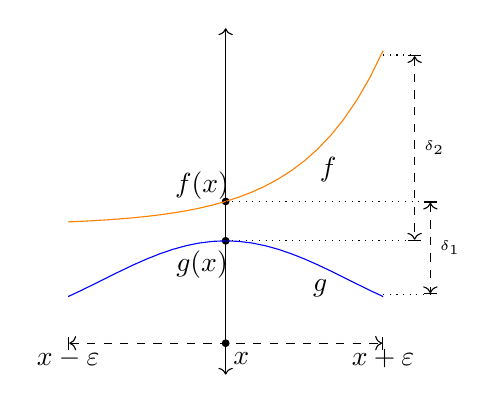
\begin{tikzpicture}[domain=-2:2]
%\draw[very thin,color=gray] (-0.1,-1.1) grid (3.9,3.9);
\draw[dashed, |<->|]   (-2,0) -- (2,0);
\draw[<->] (0,-0.4) -- (0,4); % node[above] {$f(x)$};

    \node at (0,0)[circle,fill,inner sep=1pt]{};
%    \node at (-2,0)[circle,fill,inner sep=1pt]{};
%    \node at (2,0)[circle,fill,inner sep=1pt]{};
\node(z) at (0.2,-0.2) {$x$};
\node(-e) at (-2,-0.2) {$x-\varepsilon$};
\node(e) at (2,-0.2) {$x+\varepsilon$};


\node(f) at (0,0.8+0.5)[circle,fill,inner sep=1pt]{};
\node(f) at (0,1.5+0.3)[circle,fill,inner sep=1pt]{};

\node(f) at (-0.3,2) {$f(x)$};

\node(f) at (-0.3,1) {$g(x)$};


\node(ff) at (1.3,2.2) {{$f$}};
\node(gg) at (1.2,0.7) {{$g$}};

%\draw[color=red] plot (\x,\x) node[right] {$f(x) =x$};
% \x r means to convert ?\x? from degrees to _r_adians:
\draw[color=blue] plot (\x,{0.8+ 0.5*(cos(\x r))}) ;
\draw[color=orange] plot (\x,{1.5+0.3*exp(\x)}) ;

\draw[dotted] (0,1.8) -- (2.6,1.8);
\draw[dotted] (2,0.62) -- (2.6,0.62);
\draw[dotted] (0,1.3) -- (2.4,1.3);
\draw[dotted] (2,3.66) -- (2.4,3.66);

%
%\draw[dotted] (0,1.8) -- (2, 0.62);
%\draw[dotted] (0,1.3) -- (2, 3.66);

\draw[dashed,|<->| ] (2.4,3.66) -- node[right] {\tiny$\delta_{2}$} (2.4,1.3);
\draw[dashed,|<->| ] (2.6,1.8) -- node[right] {\tiny$\delta_{1}$} (2.6,0.62);

\end{tikzpicture}
}
\caption{\small In differential logical relations the distance between two functions $f,g:\R\to \R$, computed at $(x,\varepsilon)$ is the maximum between 
$\delta_{1}=\max\{d(f(x),g(y));~ y\in [x-\varepsilon, x+\varepsilon]\}$ and 
$\delta_{2}=\max\{d(g(x), f(y));~ y\in [x-\varepsilon, x+\varepsilon]\}$.}
% and 
%
%
%minimum $\delta$ such that for all $y\in [x-\varepsilon, x+\varepsilon]$, both $g(y)\in [f(x)-\delta, f(x)+\delta]$ and $f(y)\in[g(x)-\delta, g(x)+\delta]$ hold. $\delta$ is thus $\max\{\delta_{1},\delta_{2}\}$ in the image above.}
\label{fig:graph1}
\end{subfigure} \ \ \ \ 
\begin{subfigure}{0.45\textwidth}
\parbox[h][4.6cm][c]{\textwidth}{
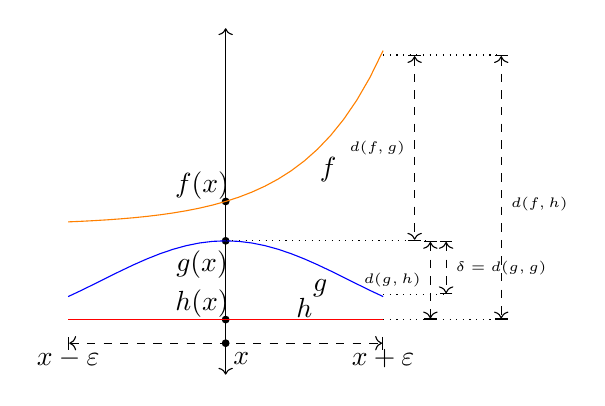
\begin{tikzpicture}[domain=-2:2]
%\draw[very thin,color=gray] (-0.1,-1.1) grid (3.9,3.9);
\draw[dashed, |<->|]   (-2,0) -- (2,0);
\draw[<->] (0,-0.4) -- (0,4); % node[above] {$f(x)$};

    \node at (0,0)[circle,fill,inner sep=1pt]{};
%    \node at (-2,0)[circle,fill,inner sep=1pt]{};
%    \node at (2,0)[circle,fill,inner sep=1pt]{};
\node(z) at (0.2,-0.2) {$x$};
\node(-e) at (-2,-0.2) {$x-\varepsilon$};
\node(e) at (2,-0.2) {$x+\varepsilon$};


\node(f) at (0,0.8+0.5)[circle,fill,inner sep=1pt]{};
\node(f) at (0,1.5+0.3)[circle,fill,inner sep=1pt]{};
\node(f) at (0,0.3)[circle,fill,inner sep=1pt]{};

\node(f) at (-0.3,2) {$f(x)$};

\node(f) at (-0.3,1) {$g(x)$};

\node(f) at (-0.3,0.5) {$h(x)$};

\node(ff) at (1.3,2.2) {{$f$}};
\node(gg) at (1.2,0.7) {{$g$}};
\node(gg) at (1,0.45) {{$h$}};

%\draw[color=red] plot (\x,\x) node[right] {$f(x) =x$};
% \x r means to convert ?\x? from degrees to _r_adians:
\draw[color=blue] plot (\x,{0.8+ 0.5*(cos(\x r))}) ;
\draw[color=orange] plot (\x,{1.5+0.3*exp(\x)}) ;
\draw[color=red] plot (\x,{0.3}) ;



\draw[dotted] (0,1.3) -- (2.6,1.3);
\draw[dotted] (2,0.3) -- (3.5,0.3);
\draw[dotted] (0,1.3) -- (2.4,1.3);
\draw[dotted] (2,3.66) -- (3.5,3.66);
\draw[dotted] (2,0.62) -- (2.8,0.62);

%
%\draw[dotted] (0,1.8) -- (2, 0.62);
%\draw[dotted] (0,1.3) -- (2, 3.66);

\draw[dashed,|<->| ] (2.4,3.66) -- node[left] {\tiny$d(f,g)$} (2.4,1.3);
\draw[dashed,|<->| ] (2.6,1.3) -- node[left] {\tiny$d(g,h)$} (2.6,0.3);

\draw[dashed,|<->| ] (2.8,1.3) -- node[right] {\tiny$\delta=d(g,g)$} (2.8,0.62);

%\draw[dashed,|<->| ] (3.5,2.96) -- node[above right] {\tiny$\begin{matrix}d(f,g)+d(g,h)\\ -d(g,g)\end{matrix}$} (3.5,0.3);

\draw[dashed,|<->| ] (3.5,3.66) -- node[below right] {\tiny$d(f,h)$} (3.5,0.3);

\end{tikzpicture}
}
%
\caption{\small The distance arising from differential logical relations is not a partial metric: the example above shows that $d(f,h)> d(f,g)+d(g,h)- d(g,g)$ (with all distances computed at $(x,\varepsilon)$).}% and 
%
%
%minimum $\delta$ such that for all $y\in [x-\varepsilon, x+\varepsilon]$, both $g(y)\in [f(x)-\delta, f(x)+\delta]$ and $f(y)\in[g(x)-\delta, g(x)+\delta]$ hold. $\delta$ is thus $\max\{\delta_{1},\delta_{2}\}$ in the image above.}
\label{fig:graph2}
\end{subfigure}
\caption{Differential logical relations do not yield partial metrics.}
\end{figure}

\subparagraph*{Related work}


A primary source of inspiration for our approach was the recent work on  \emph{differential logical relations} \cite{dallago:differential-stlc}. This is a semantical framework for higher-order languages in which a type is interpreted as a set $X$ endowed with a kind of metric structure expressed by a ternary relation $\rho \subseteq X\times Q\times X$, where $Q$ is an arbitrary quantale. To our knowledge, this is the first place were the idea of varying the quantales in which distances are measured is introduced as a key ingredient to obtain a cartesian closed category.

While the relation $\rho$ of a GMS induces a distance function $d_{\rho}(x,y)=\sup\{\varepsilon\mid \rho(x,\varepsilon,y)\}$, this function is not a (partial) metric. We can show this fact with a simple example: in this model the distance between two programs 
 $f,g:\mathsf{Real}\to \mathsf{Real}$ is taken in the quantale of functions from $\R\times \R_{+}^{\infty}$ to $\R_{+}^{\infty}$: intuitively, 
  $d(f,g)$ associates a closed interval $[x-\varepsilon,x+\varepsilon]$ (corresponding to the pair $(x,\varepsilon)$) with the smallest distance $\delta$ such that $[ f(x)-\delta, f(x)+\delta]$ and $[g(x)-\delta,g(x)+\delta]$ both contain the images of $[x-\varepsilon, x+\varepsilon]$ through
 $g$ and $f$ respectively (see Fig. \ref{fig:graph1}). Then, as shown in Fig. \ref{fig:graph2}, by letting $\delta=d(g,g)(x,\varepsilon)$, we have that $d(g,g)$ sends the interval $I=[x-\varepsilon, x+\varepsilon]$ onto the interval $[g(x)-\delta, g(x)+\delta]$, which has diameter $2\delta$, while the image of $I$ has diameter $\delta$, making the triangular law of partial metrics fail. 



Westbrook and Chaudury \cite{chaudhuri} have introduced a more syntactic approach to approximate program transformations through a System F-based type system with a type of real numbers and an explicit distinction between exact and approximate programs.
%, and provides typing rules to formalize contextual reasoning about program differences. 
%The latter are taken as functions relating errors in input and errors in output, but the viewpoint of program metric is not considered.
Most examples of contextual reasoning from \cite{chaudhuri} can be  reformulated in our framework (as the case of loop perforation discussed in Section 4). 



The literature on program pseudo-metrics is vast. A major distinction can be made between those approaches in which metrics account for \emph{extensional} aspects of programs (like ours), 
 and approaches in which metrics are used to characterize more \emph{intensional} aspects.
To the first family belong all metric models developed for reasoning about differential privacy \cite{10.1145/1932681.1863568, 10.1007/978-3-642-29420-4_3, Barthe_2012},  
probabilistic computation \cite{10.1109/LICS.2015.64, 10.1007/978-3-662-54434-1_13} and co-inductive models \cite{DESHARNAIS2004323, VANBREUGEL2005115, 10.1007/978-3-662-44584-6_4,10.1007/3-540-48224-5_35}.
%In particular, several approaches like \cite{} emphasize the importance to formalize contextual reasoning, wich can be assured in frameworks like \cite{} by the restriction to Lipschitz-continuous or non-expansive functions. 
To the second class belong approaches like \cite{Escardo1999} which recovers the Scott model of PCF through a ultrametric semantics, and most models based on partial metric spaces \cite{Bukatin1997,doi:10.1111/j.1749-6632.1994.tb44144.x}, which rely on a correspondence between continuous Scott domains and the $T_{0}$ topology of partial metrics.

From a more mathematical viewpoint, 
\cite{Stubbe2009} discusses a characterization of exponentiable GPMS, showing in particular that no such category can both be cartesian closed and contain the standard metric on $\mathbb R$. This result seems to add further evidence of the necessity of considering metrics over varying quantales in order to model higher-order languages. 
Finally, the elegant categorical approach to GPMS based on \emph{quantaloid-enriched categories} from \cite{Stubbe2018} seems to provide the relevant structure to develop explicit typing rules for our approximate programs.

%
% approach might provide good 
%categorical insights to improve our present understnd of program distances.

%
%. 
%The central motivation such approaches is the observation that a partial metric $d$ on a set $X$ induces an order relation given by $x\preceq_{d}y$ iff $d(x,y)\leq d(x,x)$, turning $X$ into a continuous Scott domain and, conversely, any continuous Scott domain with a countable basis is induced by a partial metric in this way.
%This allows to reformulate several classical results on denotational semantics using the $T_{1}$ topology of partial metric spaces.
%


%
%While in all these results distances are computed over a \emph{fixed} quantale, the generalization of this categorical approach to varying quantales seems to be a yet unexplored research direction.






\subparagraph*{Future work}


%
%
%In this paper we constructed a (non-extensional) model of the simply typed $\lambda$-calculus based on generalized partial metric spaces. Our model provides a 
% differential semantics of higher-order programs, that is, a semantic description of \emph{differences} between
% higher-order programs. 
% The main novelty is that we take as morphisms between metric spaces approximate functions, \emph{i.e.} monotone functions over intervals, rather than continuous functions of some kind. While approximate functions represent sets of similar programs, usual, exact, programs can be embedded in the model through a differentiation operator. 
% This approach allows us to overcome the well-known obstacle that usual categories of metric spaces and continuous functions are not cartesian closed, and therefore cannot be models of $\STLC$.
%% 
% Instead, we obtain 
%based on generalized partial metric spaces and
%
%Moreover, our model refines previous notions of program distances based on differential logical relations.
%
%
%the use of partial metric spaces, a well-investigated metric structure to which most fundamental properties and results on standard metric spaces scale well, 
%
%
%
%
%. More importantly, we take, as morphisms between them, approximate functions, that is, function over closed intervals, rather than (Lipschitz-) continuous or non-expansive functions over points, as in usual categories of metric spaces.

The approach we presented lends itself to further extensions and generalizations.
First, we would like to investigate the interpretation of more type constructions than those of $\STLC$ (\textit{e.g.} coproducts, recursive types, effects). Moreover, we would like to explore the possibility of exploiting the structure of the category $\dsp(\mathbb C)$ to construct new and more refined notions of approximations.
For example (we work in $\dsp(\set)$ for simplicity), 
starting from the ``standard'' set of approximate values $\mathcal I$ on $\mathbb{R}^{X\times X}$ (with elements of $\mathcal I$ being  families of compact intervals $U_{x,x'}\subseteq \mathbb R$ indexed by elements of $X$ and $X'$), one can define a new family  $\Delta^{*}\mathcal I$  of approximate values for  $\mathbb R^{X}$ by ``pulling back'' the exact map 
$\Delta:
\mathbb R^{X} \to \mathbb R^{X\times X}$ defined by $\Delta f(x,x')=f(x')-f(x)$, \textit{i.e.} letting $\Delta^{*}\mathcal I = \{ \Delta^{-1}(a) \mid a \in \mathcal I\}$. 
The new approximate values then correspond to sets of functions $f\in \mathbb R^{X}$ with a controlled variation, that is, such that $f(x')-f(x)$ is bounded by some family of intervals $U_{x,x'} \in \mathcal I$.





%
%First, in this paper we restricted our attention to $\STLC$, which is not a universal language. 
%The accommodation of full recursion in metric models is usually obtained by an application of the Banach fixed point theorem \cite{VANBREUGEL20011}. As this theorem scales well to partial metric spaces \cite{Samet:2013aa}, a natural question is whether our model, or some variant of it, can be used to provide a metric account of universal computation over the real numbers.
%


Another interesting research direction concerns probabilistic extensions of $\STLC$. 
Probabilistic metrics \cite{1029849,KOZEN1981328, 10.1109/LICS.2015.64, 10.1007/978-3-662-54434-1_13} have been the object of much research in recent years, due to the relevance of metric reasoning in some areas of computer science in which probabilistic computation plays a key role (\textit{e.g.} in cryptography \cite{GOLDWASSER1984270} and machine learning \cite{krause08robust}).
A convenient starting point seems to be the recent generalization of {probabilistic (generalized) metric spaces} to the partial metric case \cite{HE201999}.







%sdafdsf

\bibliography{CSL2021.bib}

%
%\appendix
%
%\section{Generalized partial metric spaces}
%
%dfsdfs
%
%\section{Cartesian lax-closed categories}
%
%fadfs
\end{document}
